% !TeX document-id = {1ab4115c-5a48-37e6-26a7-eb5f8e718844}
% !TeX TXS-program:compile = pdflatex -synctex=1 -interaction=nonstopmode -output-directory=build -jobname=p5_aionfpga_report_canzani_mueller report.tex
% !TeX TXS-program:bibliography = biber --output-directory build p5_aionfpga_report_canzani_mueller
% !TeX TXS-program:glossary = makeglossaries -d build p5_aionfpga_report_canzani_mueller
% !TeX TXS-program:view = txs:///view-pdf ./build/p5_aionfpga_report_canzani_mueller.pdf

\documentclass[final]{fhnwreport}

%% Packages
% Main packages
\usepackage[english]{babel}
\usepackage[T1]{fontenc}
\usepackage[utf8]{inputenc}
\usepackage{lmodern}
\usepackage{textcomp}
\usepackage{graphicx}
\usepackage{float}

% Useful packages
\usepackage[pdftex,dvipsnames,table,tables]{xcolor}
\usepackage{csquotes}
\usepackage{siunitx}
\usepackage{xfrac}
\usepackage{listings}
\usepackage{lstautogobble}
\usepackage[bottom]{footmisc}
\usepackage{footnote}
\usepackage{verbatim}
\usepackage[textsize=footnotesize]{todonotes}
%\usepackage{xurl}
%\usepackage{url}
%\usepackage{soul}

% TikZ packages
%\usepackage{standalone}
%\usepackage{tikz}
%\usepackage{circuitikz}
%\usetikzlibrary{arrows}
%\usetikzlibrary{calc}
%\usetikzlibrary{intersections}

% Math packages
\usepackage{amsmath}
%\usepackage{amssymb}
\usepackage{array}
%\usepackage{amsthm}

% Table packages
\usepackage{tabularx}
%\usepackage{longtable}
\usepackage{multirow}
\usepackage{multicol}
\usepackage{booktabs}

% Figure packages
%\usepackage{subfig}
\usepackage{caption}
\usepackage{subcaption}

% PDF packages
\usepackage{pdfpages}
\usepackage{pdflscape}

% Other packages
%\usepackage{xargs}

%% Settings
% Bibliography
\usepackage[style=ieee,dashed=false,urldate=comp,backend=biber]{biblatex}
\addbibresource{literature/bibliography.bib}

% Glossary
\usepackage[toc]{glossaries}
\makeglossaries
\input{header/glossary}

% Graphics
\graphicspath{{./graphics/}}

% Listings
% purple {0.776,0.584,0.776} / yellow {0.976,0.682,0.341} / orange {0.976,0.482,0.341}
\definecolor{keywordcolor}{rgb}{0.925,0.376,0.4} % red
\definecolor{commentcolor}{rgb}{0.651,0.675,0.725} % gray
\definecolor{stringcolor}{rgb}{0.6,0.78,0.58} % green
\definecolor{backgroundcolor}{rgb}{0.976, 0.98, 0.98} % light gray

\lstdefinestyle{C++}{
    autogobble,
    backgroundcolor=\color{backgroundcolor},
    commentstyle=\color{commentcolor},
    keywordstyle=\color{keywordcolor},
    numberstyle=\tiny\color{commentcolor},
    stringstyle=\color{stringcolor},
    basicstyle=\ttfamily\footnotesize,
    breakatwhitespace=false,
    breaklines=true,
    breakautoindent=true,
    breakindent=50pt,
    escapeinside={(*}{*)},
    captionpos=b,
    keepspaces=true,
    numbers=left,
    numbersep=5pt,
    showtabs=false,
    showspaces=false,
    showstringspaces=false,
    tabsize=2,
    language=C++
}


% Other
%\geometry{twoside=false}
\setlength{\marginparwidth}{2cm}
\overfullrule=5em

%% Custom definitions
% Table definitions
\newcolumntype{L}[1]{>{\raggedright\arraybackslash}p{#1}}
\newcolumntype{C}[1]{>{\centering\arraybackslash}p{#1}}
\newcolumntype{R}[1]{>{\raggedleft\arraybackslash}p{#1}}
\newcolumntype{M}[1]{>{\centering\arraybackslash}m{#1}}
\newcolumntype{N}{@{}m{0pt}@{}}

% Month
\newcommand{\MONTH}{
	\ifcase\the\month
	\or January
	\or February
	\or March
	\or April
	\or May
	\or June
	\or July
	\or August
	\or September
	\or October
	\or November
	\or December
	\fi}

% URL
\urlstyle{same}

% siunitx
\sisetup{per=fraction}



\title{\textbf{{\Huge AI High-Performance Solution \\[2mm] on FPGA}}}
\author{\textit{{\LARGE Project Report}}}
\date{}

\begin{document}

% Title page
\selectlanguage{english}
\pagenumbering{gobble}
\maketitle

\begin{figure}[H]
  \centering
  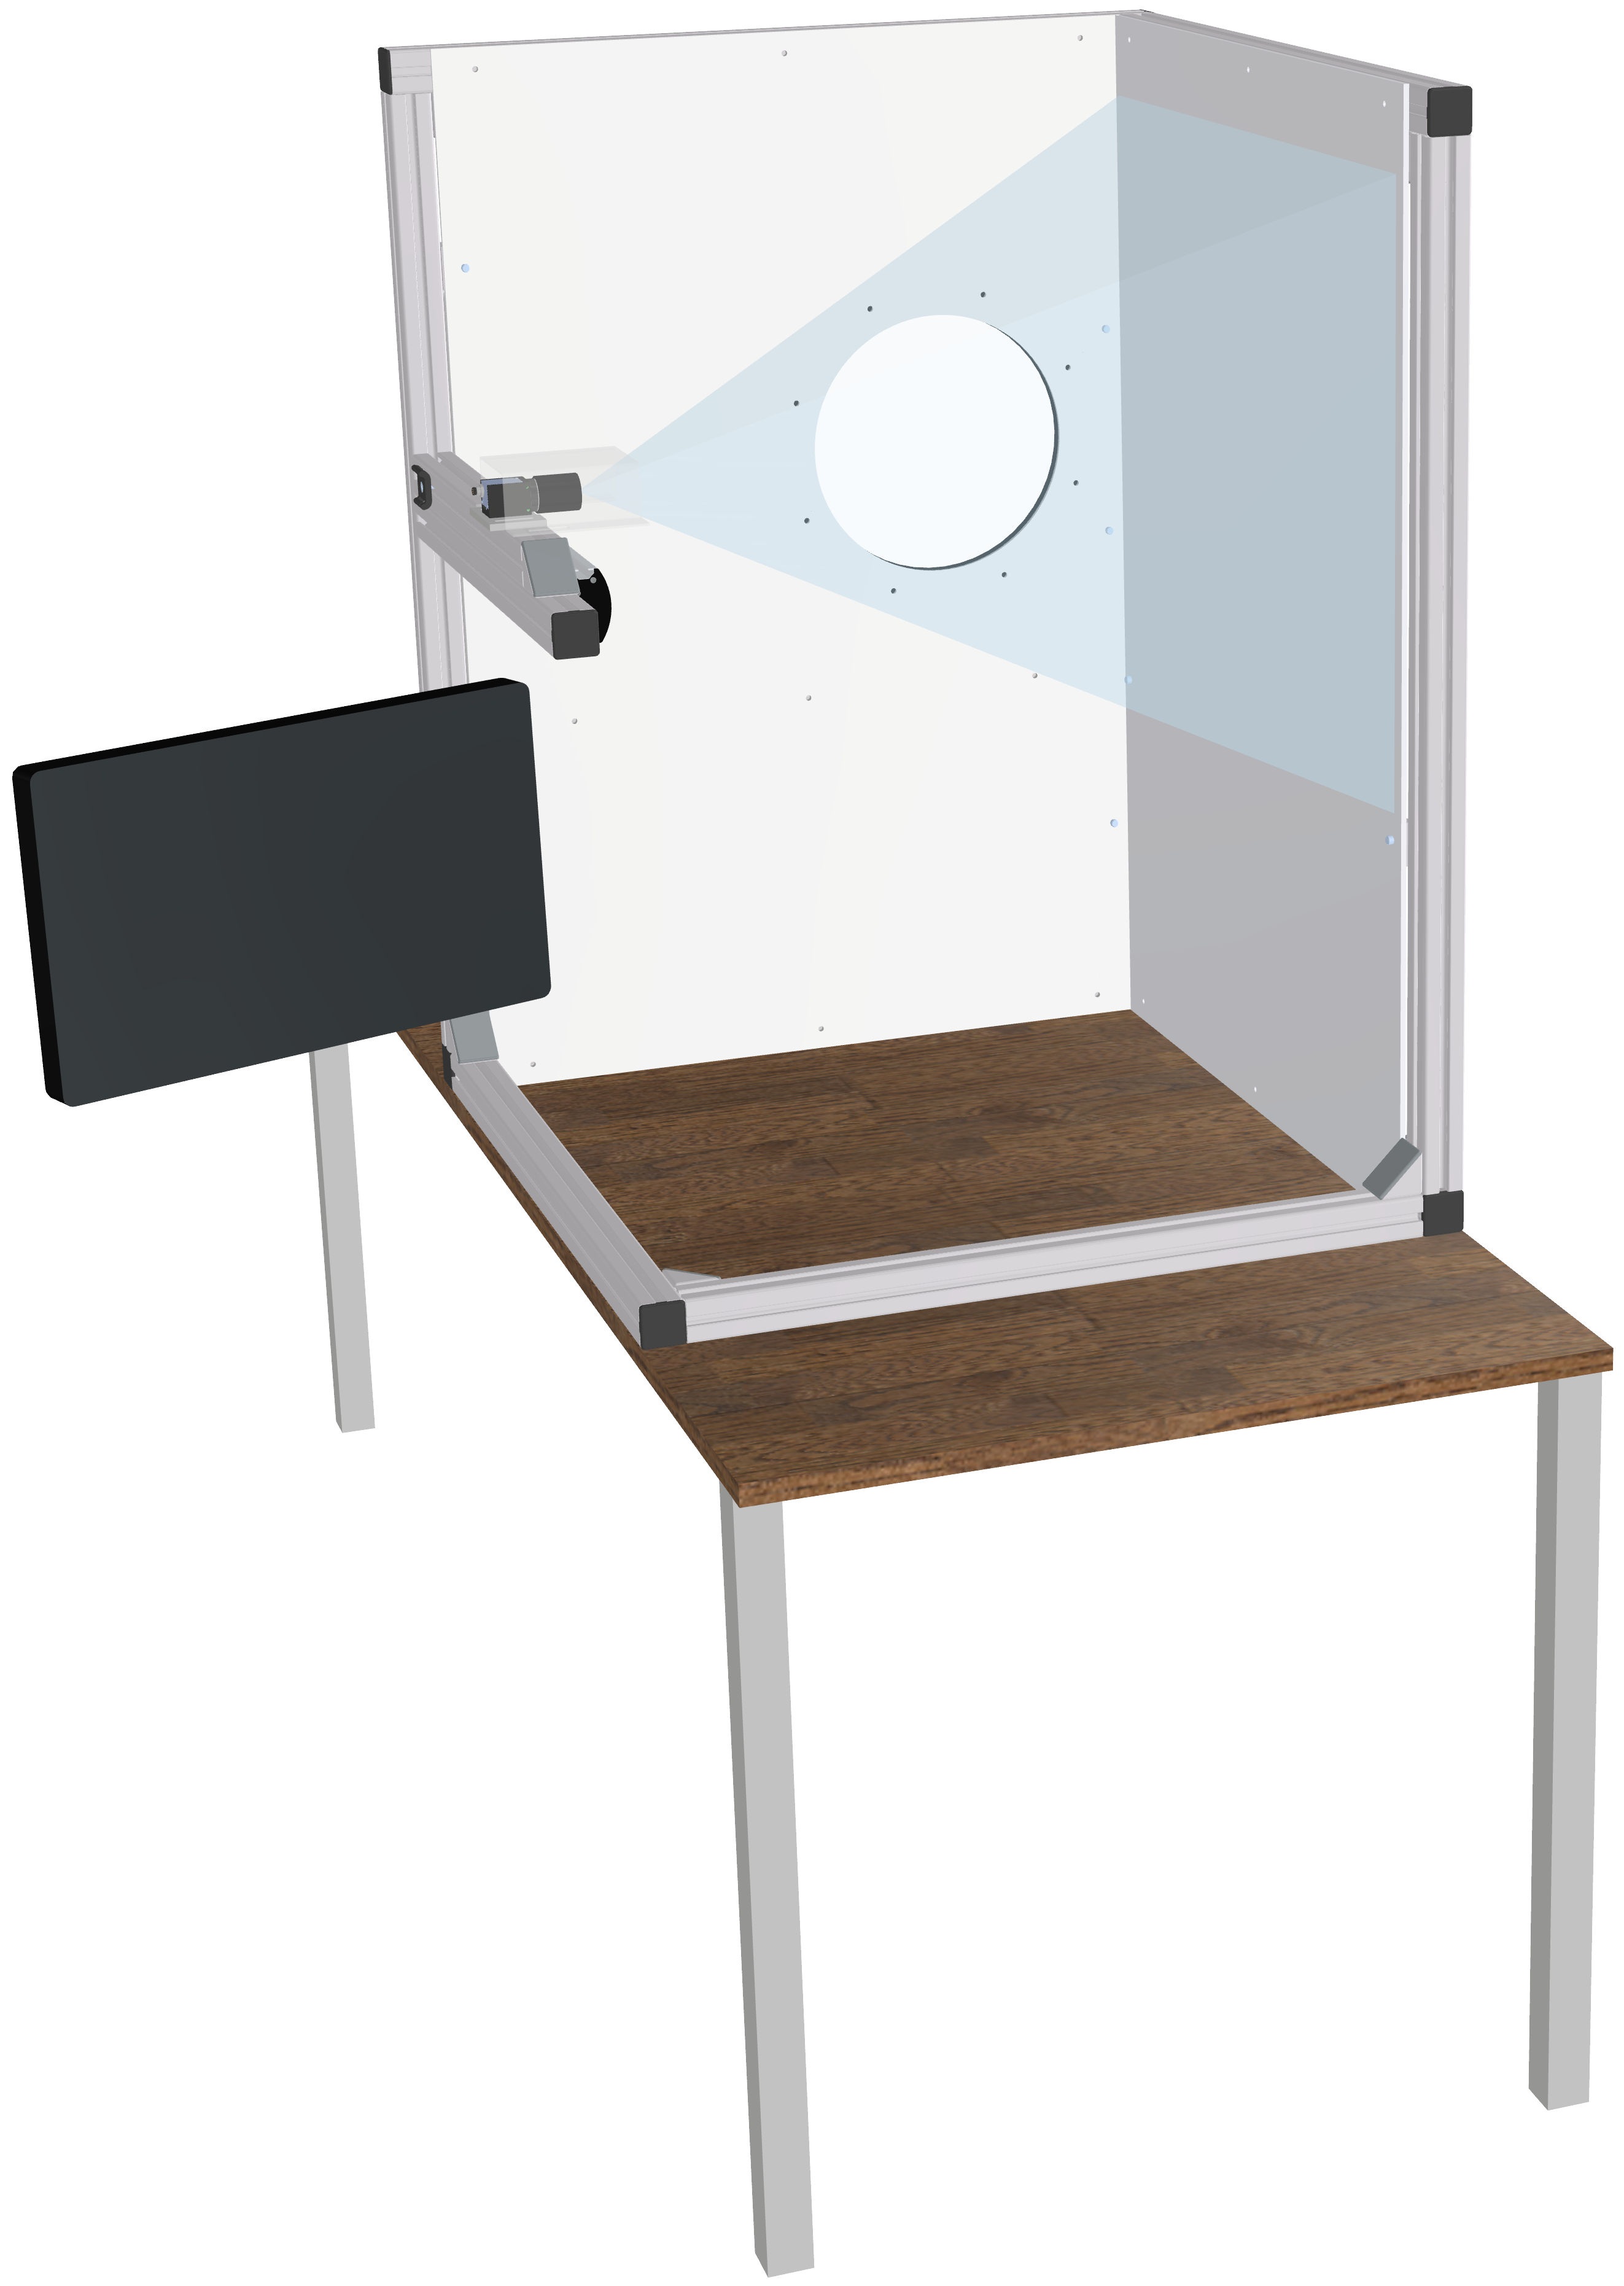
\includegraphics[width=0.55\textwidth]{top_assembly}
\end{figure}

\vfill
\begin{center}
  \begin{tabular}{>{\bfseries\large}rl}
    Degree Program & Electrical Engineering and Information Technology \\[2mm]
    Customer       & Institute for Sensors and Electronics \\[2mm]
    Coaches        & Prof. Michael Pichler, Prof. Dr. Hanspeter Schmid \\[2mm]
    Team           & Nico Canzani, Dominik M\"uller \\[2mm]
    Date           & \the\day.\MONTH \the\year
  \end{tabular}
\end{center}
\clearpage

% Abstract
\pagenumbering{roman}
% \vspace*{\fill}
% \null\vspace{\fill}
\todo{Dominik}
\begin{abstract}
\noindent Lorem ipsum dolor sit amet, consectetur adipiscing elit, sed do eiusmod tempor incididunt ut labore et dolore magna aliqua. Ut enim ad minim veniam, quis nostrud exercitation ullamco laboris nisi ut aliquip ex ea commodo consequat. Duis aute irure dolor in reprehenderit in voluptate velit esse cillum dolore eu fugiat nulla pariatur. Excepteur sint occaecat cupidatat non proident, sunt in culpa qui officia deserunt mollit anim id est laborum.

% Motivation
% Problem statement
% Approach
% Results
% Conclusions
% from https://users.ece.cmu.edu/~koopman/essays/abstract.html

\vspace{3em}
\begin{tabular}{>{\bfseries}ll}
  Team members  & Nico Canzani, Dominik M\"uller \\
  Keywords      & Keyword1, Keyword2, Keyword3
\end{tabular}
\end{abstract}
% \vspace*{\fill}
% \vspace{\fill}

\clearpage

% Contents
\tableofcontents
\clearpage

% Sections
\pagenumbering{arabic}
\section{Introduction}
\label{sec:introduction}
%Die technische Welt befindet sich in einem ständigen Wandel. Eine der gewichtigsten Neuerungen ist die Künstliche Intelligenz, oder kurz KI genannt.
%Künstliche Intelligenz ist der Grundbaustein diverser Grossunternehmen, wie beispielsweise Google oder Facebook.
%Auch bei den Privatpersonen hat die KI Einzug gehalten.
%Fei-Fei Li, Professor of Computer Science at Stanford University sagte mal:
% 	Zitat
The technical world is in a constant state of change. One of the most important innovations is artificial intelligence, or AI for short.
Artificial intelligence is the basic building block of various large companies, such as Google or Facebook.
AI has also found its way into the world of private individuals.
Fei-Fei Li, Professor of Computer Science at Stanford University said once:
\begin{quote}
	"I imagine a world in which AI is going to make us work more productively, live longer, and have cleaner energy."\cite{quotes_future}
\end{quote}
This scenario has already started. As an example of what artificial intelligence is capable of, the above paragraph was translated from a German text using the artificial intelligence of DeepL. The result is impressive.
However, AI is very versatile. In medicine, it is used to diagnose, cars should be able to drive independently or banks can recognize unauthorized use of credit cards \cite{artificial_intelligence_a_modern_approach}.
AI is used in nearly every industry and has become an important business factor.

Another challenge in today's world is the increasing data volume. More and more data should be processed in the shortest possible time. This makes fast hardware indispensable.

Project 5, AI High-Performance Solution, covers two topics, artificial intelligence and fast data processing.
A demo object for trade fairs is to be developed in which artificial intelligence is implemented on a field-programmable gate array (FPGA).
The demo object will be shown at exhibitions and represents the Fachhochschule Nordwestschweiz (FHNW).
It is a throwing booth, which is able to detect and recognize flying objects working standalone.

An Ultra96-V2 Development Board serves as hardware.
Its multiprocessor system-on-chip (MPSoC) used there, an UltraScale+ MPSoC ZU3EG, has arm-based microprocessors and an FPGA.

The first step is to create the basic conditions for designing an AI.
This is, on the one hand, the throwing booth and, on the other hand, a dataset. A dataset is needed to train a neural network.
In addition, project 5 includes an introduction to the field of artificial intelligence.
In project 6, based on project 5, artificial intelligence will be implemented on the Ultra96 board.

This technical report describes the theoretical and technical principles needed to implement the project.
\section{Artificial Intelligence}
\label{sec:ai}
% \todo[inline]{Citations}

Artificial intelligence (AI) is a branch of computer science that deals with the simulation of intelligent behaviour in computers.
Machine Learning (ML) is a subfield of AI and deals with the study of algorithms that computers use to perform certain tasks without using explicit instructions.
Deep learning is a family of machine learning methods which are based on artificial neural networks (ANNs).
A convolutional neural network (CNN) is a specific deep learning architecture that is primarly used for image classification.
% https://pathmind.com/wiki/ai-vs-machine-learning-vs-deep-learning

This chapter provides a brief overview of ML and a short introduction to CNNs.
% This chapter provides a brief overview of machine learning and CNNs.

\subsection{Machine Learning}
\label{subsec:ml}
% \todo[inline]{Citations}

As previously mentioned, machine learning is a branch of artificial intelligence that essentially aims to give computers the ability to learn from data.
The best results are achieved by using deep learning architectures in combination with large datasets.
% https://pathmind.com/wiki/neural-network

There exist different types of learning such as supervised and unsupervised learning.

\paragraph{Supervised Learning}
Supervised learning uses labeled datasets to learn.
The algorithm takes a guess on a piece of data from the dataset and this guess is then checked against the label (i.e. the correct answer).
This enables the algorithm to adjust itself and therefore to make it guess better.
% https://pathmind.com/wiki/supervised-learning

\paragraph{Unsupervised Learning}
Unsupervised learning works with unlabeled data and thus only operates with the input data.
The algorithm must learn to make sense of the input data, as it has no means of correcting itself.
Unsupervised learning is usually used in problems that involve finding groups in data or summarizing the distribution of data.
The majority of all data is not labeled and therefore the potential of unsupervised learning is enourmous.
The improvement of unsupervised learning is essential for the future of artificial intelligence.
% https://pathmind.com/wiki/unsupervised-learning

\subsection{Convolutional Neural Network}
\label{subsec:cnn}
% \todo[inline]{Citations}

Convolutional neural networks are a type of deep learning architecture that is primarily used to classify images.
They are based on artificial neural networks and the mathematical convolution operation.
The efficiency in image classification of CNNs is largely responsible for the reputation of deep learning \cite{cnn_pathmind}.

The main problems when working with color images is that they are high-dimensional and therefore require a lot of processing power.
For this reason, convolutional neural networks use special layers to detect features and reduce the amount of data.
The three different layers used are convolution layers, pooling layers and fully-connected layers.
% An example of a CNN sequence to classify handwritten digits is shown in figure \ref{fig:cnn}.
Figure \ref{fig:cnn} shows an example of a CNN sequence to classify handwritten digits \cite{cnn_pathmind}.

\paragraph{Convolution Layer}
The convolution layer performs the convolution operations using so-called kernels or filters.
The goal of the convolution operation is to extract certain features --- such as edges --- from the image.
Different kernels are used to detect different features.
The first convolution layers are responsible for capturing low-level features, while following layers are responsible for capturing high-level features \cite{cnn_tds}.
\clearpage

\paragraph{Pooling Layer}
Pooling layers reduce the spatial size of the convolved features.
Pooling is done by only looking at the portion of the image masked by the kernel.
Maximum pooling yields the maximum value and average pooling yields the average value of the masked portion.
By doing so, the required computational power is significantly decreases and the dominant features are extracted \cite{cnn_tds}.
\\

\paragraph{Fully-Connected Layer}
The fully-connected layers are responsible for learning the non-linear combinations of the high-level convolved features.
They flatten the result of the convolution process into a vector of values.
Each value corresponds to the probability that a certain feature belongs to a label \cite{cnn_tds}.
% Each value corresponds to a probability that a certain feature belongs to a label \cite{cnn_tds}.
% Each value corresponds to a probability that a certain feature belongs to a certain label \cite{cnn_tds}.

\begin{figure}[t]
  \centering
  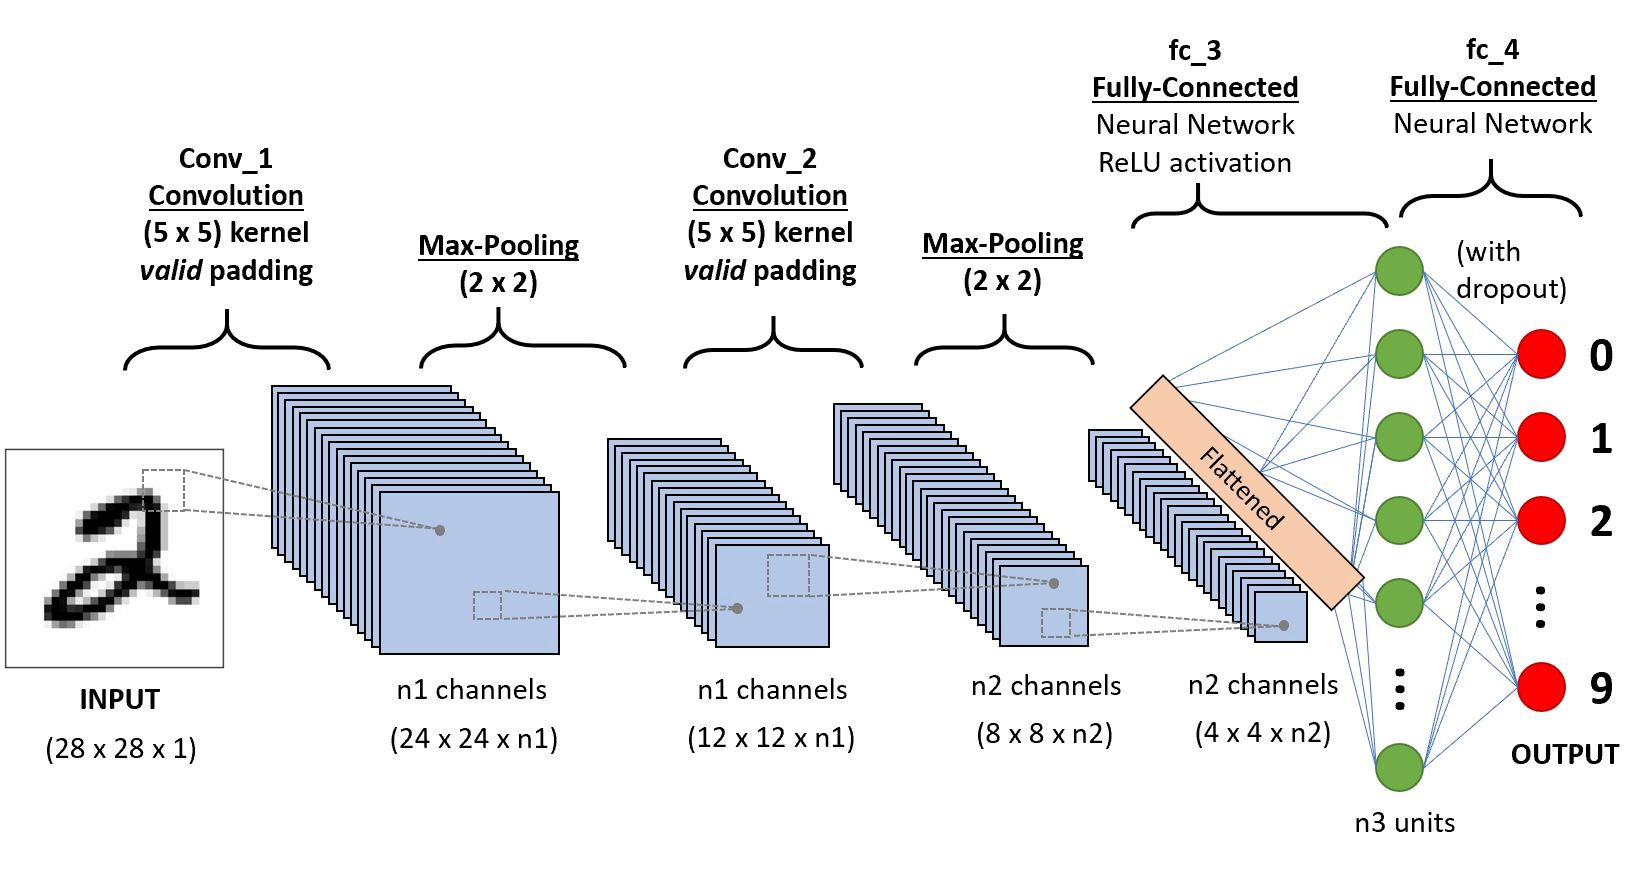
\includegraphics[width=\textwidth]{cnn}
  \caption{Example of a convolutional neural network \cite{cnn_tds}}
  \label{fig:cnn}
\end{figure}


\section{MPSoC Development Board}
\label{sec:board}

The hardware is an Ultra96-V2 board, which is distributed by Avnet.
The MPSoC installed on it is a Xilinx Zynq UltraScale+ MPSoC ZU3EG A484.
This chip is from the Zynq UltraScale+ family and has an UltraScale architecture.
Integrated is a Quad-core ARM Cortex A53 processor to run a complete operating system and a Dual-core ARM Cortex R5, which makes the Ultra96-V2 hard realtime capable.
The A53 core can be clocked with \SI{1.5}{GHz}, the R5 with \SI{600}{MHz}.

The FPGA on the MPSoC allows a hardware acceleration of up to a factor of 20 compared to the fastest CPUs \cite{acceleration_xilinx}.
Xilinx therefore recommends the board as ideal for the field of high speed artificial intelligence \cite{ai_resources_xilinx}.
The most important specifications of the MPSoC are listed in table \ref{tab:specs_MPSoC}.

\begin{table}[h]
	\caption{Specification of the Xilinx Zynq UltraScale+ MPSoC ZU3EG A484 \cite{xilinx_zynq}}
	\label{tab:specs_MPSoC}
	\centering
	\begin{tabular}{ll}
		\toprule
		& \textbf{MPSoC} \\
		\midrule
		\textbf{Logic Cells} & \SI{154}{k} \\
		\textbf{Flip Flops} & \SI{141}{k} \\
		\textbf{Block RAM} & \SI{7.6}{Mb} \\
		\textbf{DSP Slices} & 360 \\
		\bottomrule
	\end{tabular}
\end{table}

The Ultra96-V2 also features two USB 3.0 ports and a \SI{2}{GB} low-power double data rate 4 (LPDDR4) RAM, which are essential for fast image processing.
A mini DisplayPort serves as a connection to a monitor \cite{avnet_ultra96v2}.
This guarantees a standalone operation.

\section{Throwing Booth}
\label{sec:booth}
The booth is constructed from Item Profiles.
The objects are thrown through in front of a constant background, therefore there is a white back wall opposite the camera.
When creating the booth design, care was taken to ensure that the size corresponds to the width of a table (750mm).
This also defined the distance between the camera and the back wall.
With the opening angle of the lens, the minimum required size of the back wall can be calculated as in equation \ref{eq:Fieldwith}. 
In the following this size is called field of view.

\begin{equation}
	f_\text{w} = 2 \cdot a \cdot \tan\left( \frac{\vartheta}{2}\right) = \SI{690}{mm}
	\label{eq:Fieldwith}
\end{equation}

Whereby the following applies:
\begin{itemize}
	\item $f_\text{w}$ = width of the field of view
	\item $a$ = Distance camera to back panel = \SI{630}{mm}
	\item $\vartheta$ = horizontal angle of view = \SI{57.4}{\degree} \cite{baumer_lense}
\end{itemize}

Assuming that the picture format is 1280 $\times$ \SI{1024}{px}, the height of the field of view ($f_\text{h}$) is equal to

\begin{equation}
	f_\text{h} = f_\text{w} \cdot \frac{\SI{1024}{px}}{\SI{1280}{px}} = \SI{552}{mm}.
	\label{eq:Fieldhight}
\end{equation}

The objects should be passed as far away from the camera as possible to be able to take more pictures per throw.
To ensure that the objects are thrown through the field of view and far away from the camera, there is a hole in the back wall as a target.
It is located on the right side of the back wall, which is further away from the camera.
If the throwing objects are hit through the hole in the rear wall, they land in a net.

The back wall is made of a 5 mm thick plate of ABS.
This material is robust and withstands the impacts of the throwing objects.
The side wall is made of foamed PVC.
Due to the manufacturing process, the plate is less smooth, which results in less light reflections and therefore better pictures.

The whole throwing booth is drawn in the CAD tool Inventor. It is designed with all its components using a 3D model.
The camera is mounted on an Item profile with an aluminum mounting adapter which is shown in figure \ref{fig:mounting_adapter} and protected from damage with an aluminum sheet.
Both components have slotted holes to allow fine adjustments to be made during assembly.
The drawings of these parts can be found in the appendix \ref{app:drawings_camera_protection} and \ref{app:drawings_mounting_adapter}.

\begin{figure}[h]
	\centering
	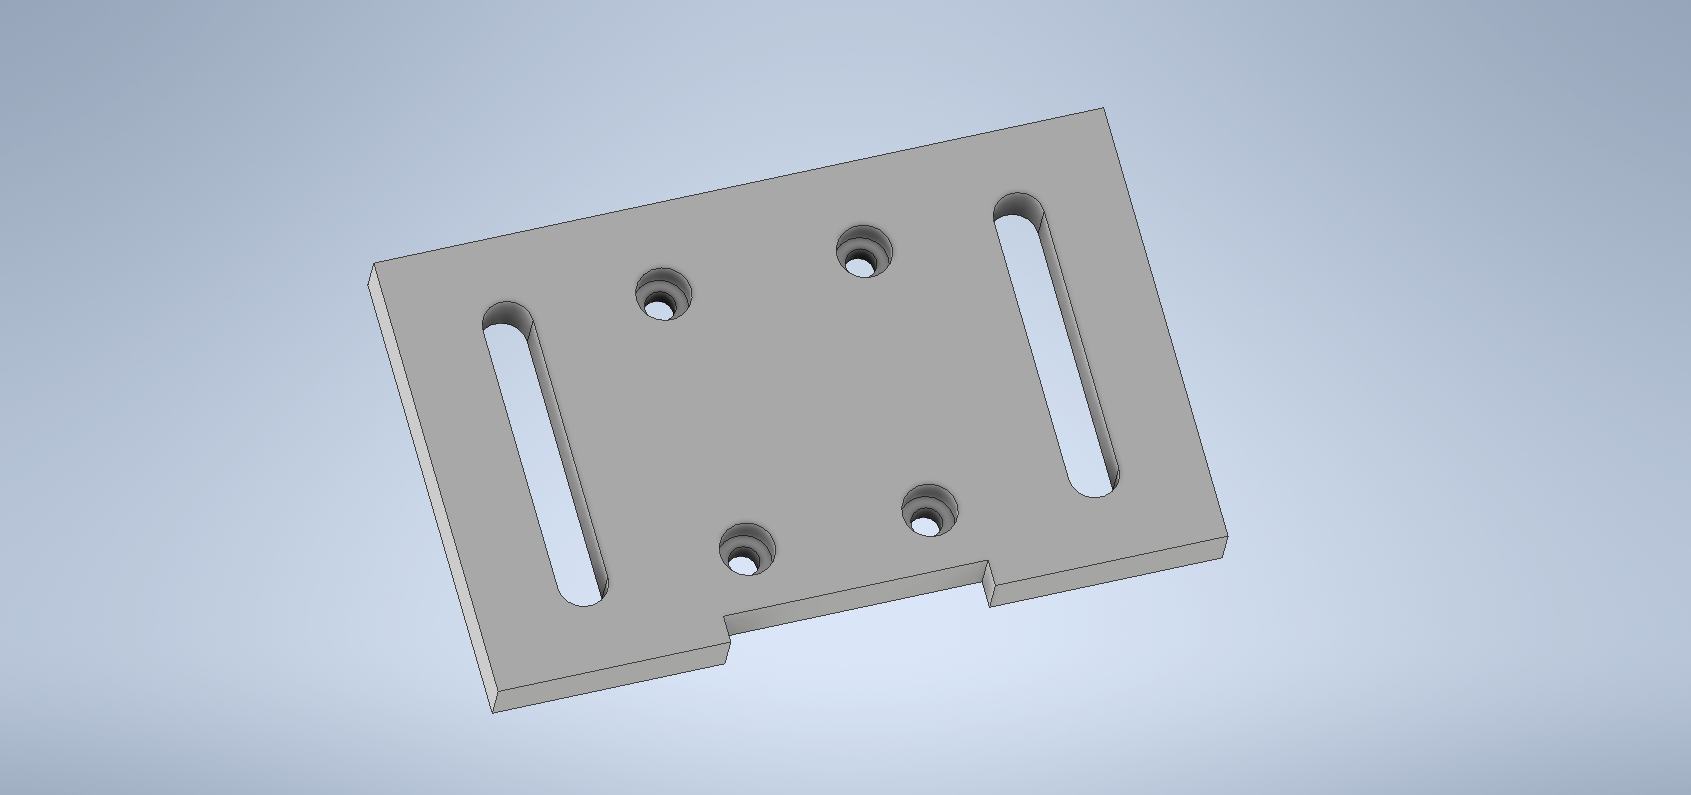
\includegraphics[width=0.4\textwidth]{graphics/mounting_adapter.png}
	\caption{Camera mounting adapter}
	\label{fig:mounting_adapter}
\end{figure}

The power supplies for all electronic components are placed in a box together with the Ultra96-V2.
The box is a case from Fibox with a transparent cover to give visitors an impression of the way it works.
It has a \SI{230}{VAC} power cable, a \SI{24}{VDC} output for lighting, a Mini DisplayPort cable for the monitor, and the USB cable for the camera.
Further there are three fans on the walls to ensure that the Ultra96-V2 is cooled.
The box also contains terminal blocks and cable trunking to store cables that are too long.
Figure \ref{fig:fibox3d} shows a 3D model of the box. The construction drawings for the Fibox case can be found in the appendix \ref{app:drawings_fibox_bottom}.

\begin{figure}[h]
	\centering
	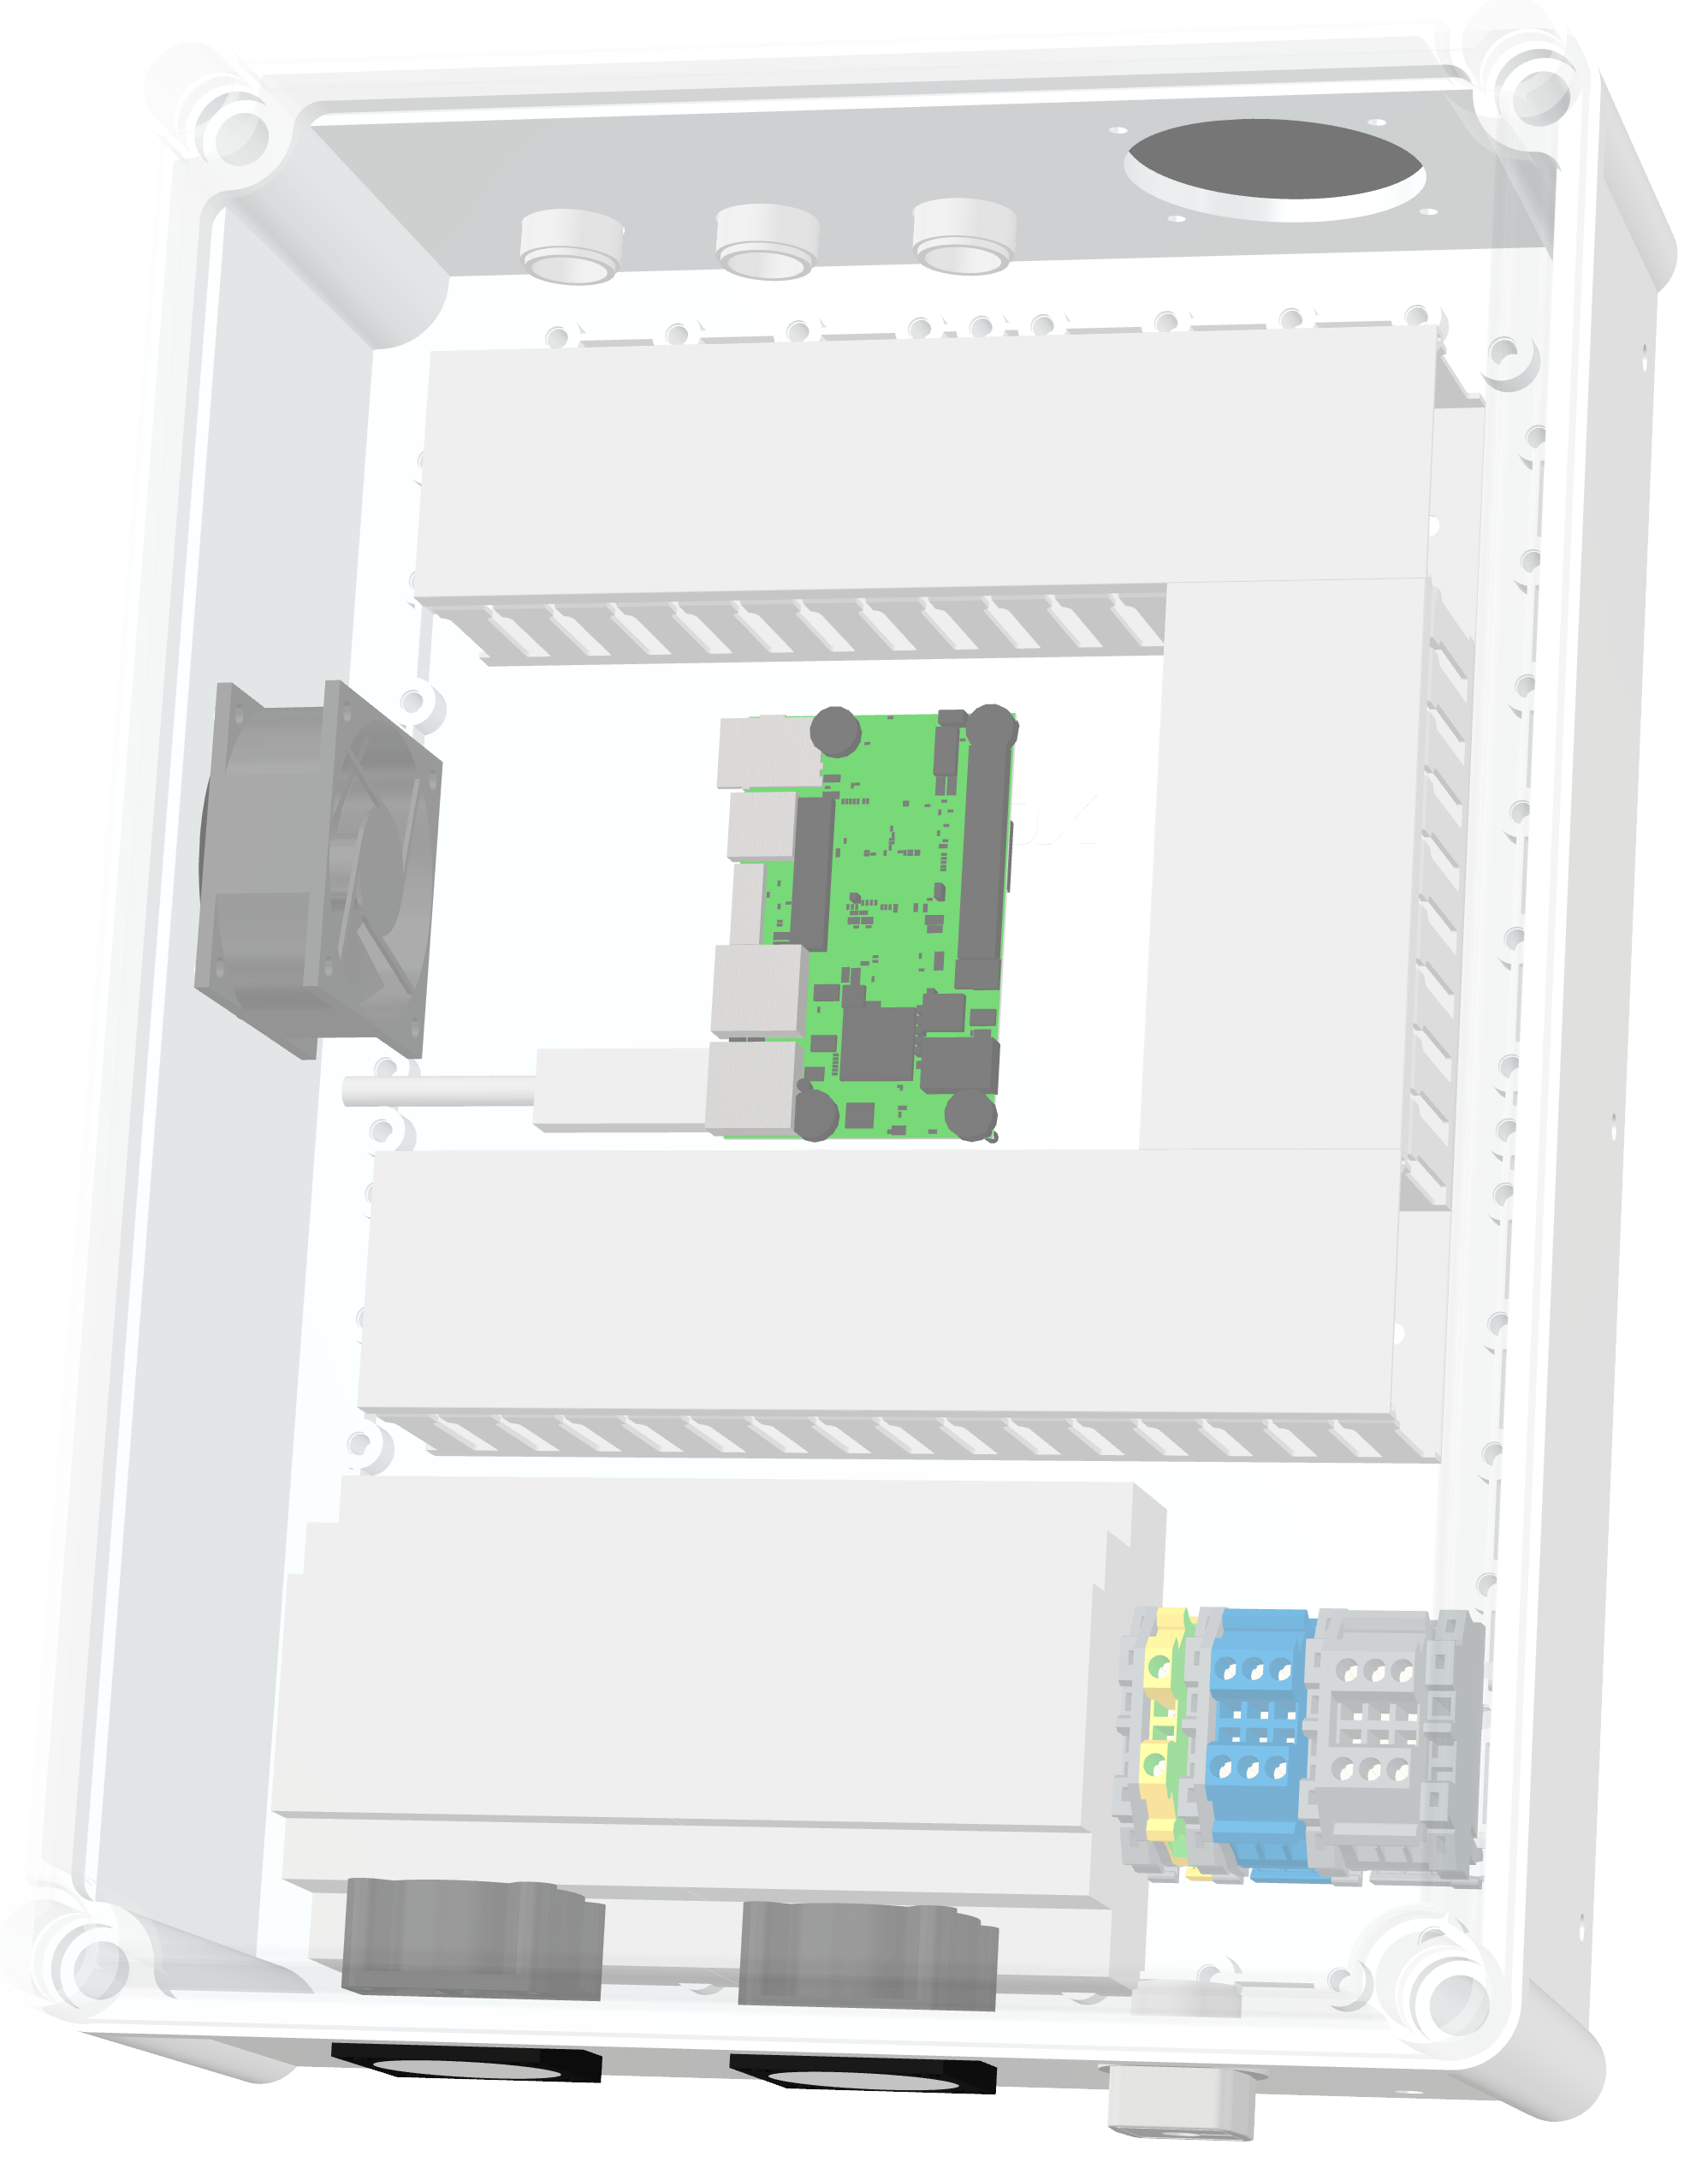
\includegraphics[width=0.3\textwidth]{graphics/case.png}
	\caption{3D Model of the Fibox case}
	\label{fig:fibox3d}
\end{figure}
\section{Camera}
\label{sec:camera}
\subsection{Webcam}
\label{subsec:webcam}
A simple webcam is not enough to capture fast moving objects with sufficient quality. 
There are several reasons for this.
Firstly, certain parameters, such as the exposure time, cannot be adjusted by the user.
This would be necessary to capture the contours of the object being thrown as detailed as possible.
Secondly, conventional webcams work with a rolling shutter.
Technically this means that fewer sensors are used. Therefore one sensor processes several pixels one after the other.

This results in the rolling shutter effect when the image changes.
On the one hand this effect is noticeable when the light flickers quickly.
For example the upper part of an image can be brighter than the lower part.
On the other hand there are problems with moving pictures.
The lower part of the image was taken at a later time, so the object appears distorted \cite{global_rolling_shutter}.

To eliminate this problem, some cameras feature the global shutter. 
This takes all pixels at the same time and stores them. 
Thus no distortions in the image occur.

This can be shown well with an example.
In the figure \ref{subfig:rollingshutter} is a recording of a ball with rolling shutter. 
Figure \ref{subfig:globalshutter} shows the same object, taken with a global shutter camera.
The distortion from the rolling shutter is clearly visible and distorts the effective object.

\begin{figure}[ht]
	\centering
	\begin{subfigure}[b]{0.4\textwidth}
		\centering
		
\includegraphics[width=0.3\textwidth]{rollingshutter}
		\caption{Rolling shutter}
		\label{subfig:rollingshutter}
	\end{subfigure}
	\begin{subfigure}[b]{0.4\textwidth}
		\centering
		
\includegraphics[width=0.3\textwidth]{globalshutter}
		\caption{Global shutter}
		\label{subfig:globalshutter}
	\end{subfigure}
	\caption{Difference rolling shutter and global shutter camera \cite{shuttermode}}
	\label{fig:shuttermode}
\end{figure}

\subsection{Baumers industrial camera}
\label{subsec:baumer_cam}

In addition to the global shutter requirement, the camera must also meet other specifications.

To ensure that an image is always obtained even from fast objects, the maximum duration between two images is

\begin{equation}
  T_\text{max} = \frac{f_\text{w} \cdot 0.75}{v_\text{max}} = \frac{\SI{0.69}{m} \cdot 0.75}{\SI{30}{\frac{m}{s}}} = \SI{17.25}{ms}.
  \label{eq:needed_T}
\end{equation}

It is assumed that the object is thrown in the last quarter of the booth and the maximum throwing speed is \SI{30}{m/s}.
This speed is approximately half the speed of the fastest baseball throw and is more or less attainable for an adult with the objects present \cite{speed_baseball}.

From equation \ref{eq:needed_T} it can be seen that the camera needs a frame rate which is higher than

\begin{equation}
  f_\text{min} = \frac{1}{T_\text{max}} = \frac{1}{\SI{17.25}{ms}} = \SI{58}{fps}.
  \label{eq:needed_fps}
\end{equation}

In order to capture the contours of the objects being thrown as detailed as possible, the motion blur must be kept to a minimum. 
This can be achieved by short exposure time. 
With the assumption that the motion blur should be smaller than or equal to \SI{3}{cm}, there results a maximum exposure time of the camera of

\begin{equation}
  t_\text{exp} = \frac{s_\text{max}}{v_\text{max}} = \frac{\SI{0.03}{m}}{\SI{30}{\frac{m}{s}}} = \SI{1}{ms}.
  \label{eq:texp}
\end{equation}

In this project a VCXU-13C camera from Baumer is used.
The Baumer company produces various sensors, such as CMOS sensors with different specifications.
The VCXU-13C has global shutter.
Furthermore it has an USB 3.0 interface for data transfer.
This is required because the Ultra96-V2 does not support an Ethernet interface.
The camera's frame rate is \SI{222}{fps}, which guarantees at least three pictures of each throw.
The minimum exposure time is \SI{20}{\micro s} \cite{baumer_cam}.

The camera requires a lens as well.
Suitable for the camera is the lens ZVL-FL-HC0614-2M, which is also manufactured by Baumer.
The aperture is manually operated to focus the images.

\subsection{Lighting}
\label{subsec:Lighting}
The more light there is, the shorter the lighting time can be selected.
This results in a clearer image, which is an advantage in image recognition.
In order for the objects to be as independent of the lighting as possible, the lighting must not flicker and the field of view should be illuminated as uniformly as possible.

The SVL BAR LIGHT LHF300-WHI from Stemmer Imaging meets these requirements.
A completely uniformly illuminated image cannot be achieved with a single LED bar.
In the data sheet Stemmer specifies the illumination of a \SI{1}{m} $\times$ \SI{1}{m} image section according to graphic \ref{fig:lighting_LEDBAR}.
The distance from the camera to the measuring surface is \SI{0.5}{m}.
The green frame corresponds to the field of view.
The illumination is therefore very satisfying.

\begin{figure}[h]
	\centering
	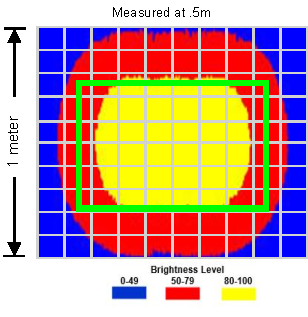
\includegraphics[width=0.3\textwidth]{graphics/brightness_level.pdf}
	\caption{Brightness Distribution according to Stemmer \cite{stemmer_datasheet}}
	\label{fig:lighting_LEDBAR}
\end{figure}
\section{Dataset}
\label{sec:dataset}
% \todo[inline]{Layout (also text arrangements!), Image of the statistics bigger or different?}

The dataset contains images of 22 different throwing objects, as shown in table \ref{tab:objects}.
It is fully labeled and consists of more than \num{15000} usable images with at least 480 images of each object.
All images were collected over the cource of two days.
Figure \ref{subfig:stuffed_bunny} shows an example image of the \textit{Stuffed Bunny} and figure \ref{subfig:hand_featherball} shows an image of the \textit{Hand Featherball}.

Figure \ref{fig:statistics} shows the statistics.
It is evident that there are generally more images of larger objects.
This is, on the one hand, due to the specific implementation of the throw detection mechanism (see section \ref{subsec:throw_detection_mechanism}).
On the other hand, the field of view is not uniformly illuminated, as described in section \ref{subsec:Lighting}.
For those reasons, a larger object area is required at the borders to achieve a sufficiently large change in the image.
However, this also leads to the fact that larger objects are more often only partially in the picture.

An important thing is that, on the first day, the white balance was performed continuously (every three images).
This caused the background color of large colored objects to be distorted.
It remains to be seen whether this will become a problem during training.
However, if this should become a problem, the respective images can easily be removed, as the labels contain a Unix timestamp (see section \ref{subsec:database}).

\begin{table}[hb]
  \caption{List of the different throwing objects}
  \label{tab:objects}
  \centering
  \begin{tabular}{lll}
    \toprule
    \textbf{Objects} &  &  \\
    \midrule
	Nerf Dart & Spiky Ball & Stuffed Bunny \\
	American Football & Tesafilm & Goalkeeper Glove \\
	Table Tennis Ball & Sponge & Hemp Cord \\
	Shuttlecock & Lego Duplo Brick (Red) & Paper Ball \\
	Sporf & Lego Duplo Brick (Green) & Beer Cap \\
	Arrow & Lego Duplo Figure & Water Bottle \\
	Hand Featherball & Foam Dice &  \\
	Floorball & Infant Shoe &  \\
    \bottomrule
  \end{tabular}
\end{table}

\begin{figure}[hb]
  \centering
  \begin{subfigure}[b]{0.45\textwidth}
    \centering
    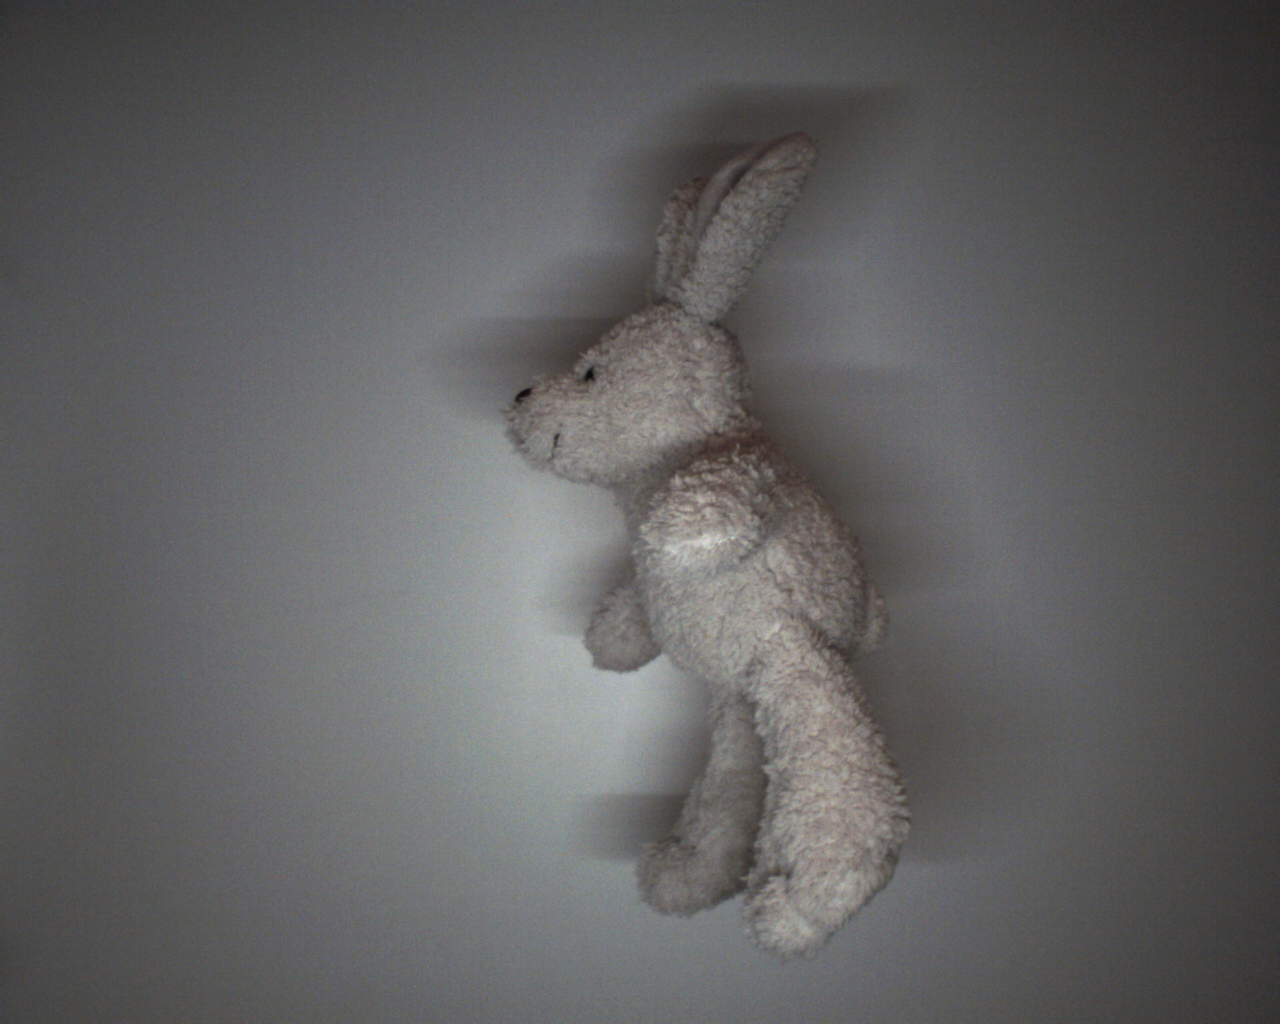
\includegraphics[width=0.9\textwidth]{1574952009_278_10_stuffed-bunny}
    \caption{Stuffed Bunny}
    \label{subfig:stuffed_bunny}
  \end{subfigure}
  \begin{subfigure}[b]{0.45\textwidth}
    \centering
    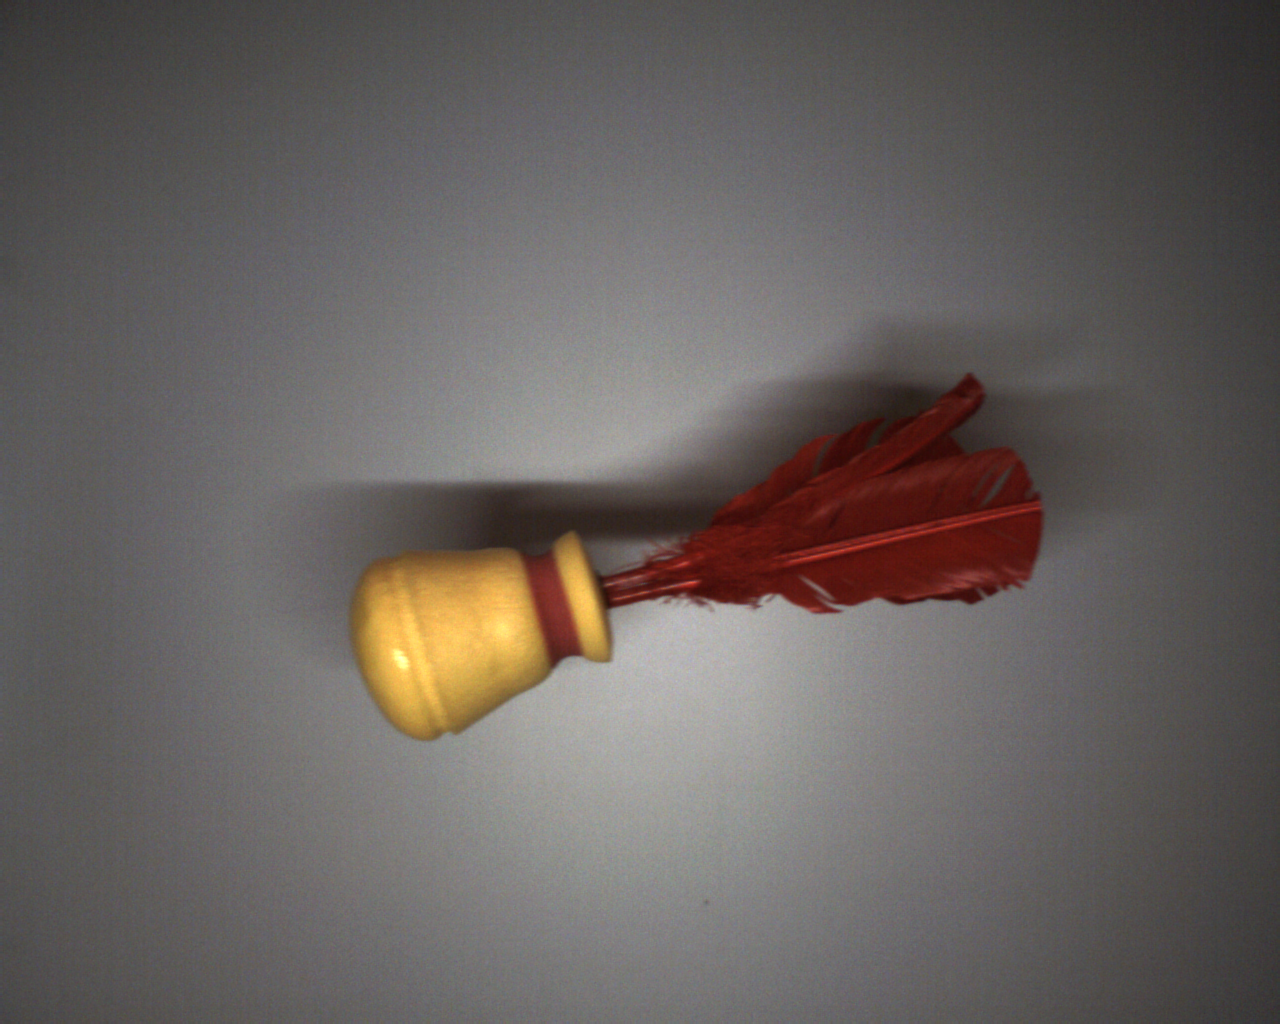
\includegraphics[width=0.9\textwidth]{1574943825_125_8_hand-featherball}
    \caption{Hand Featherball}
    \label{subfig:hand_featherball}
  \end{subfigure}
  \caption{Two pictures from the dataset}
  \label{fig:dataset}
\end{figure}

\begin{figure}[h]
  \centering
  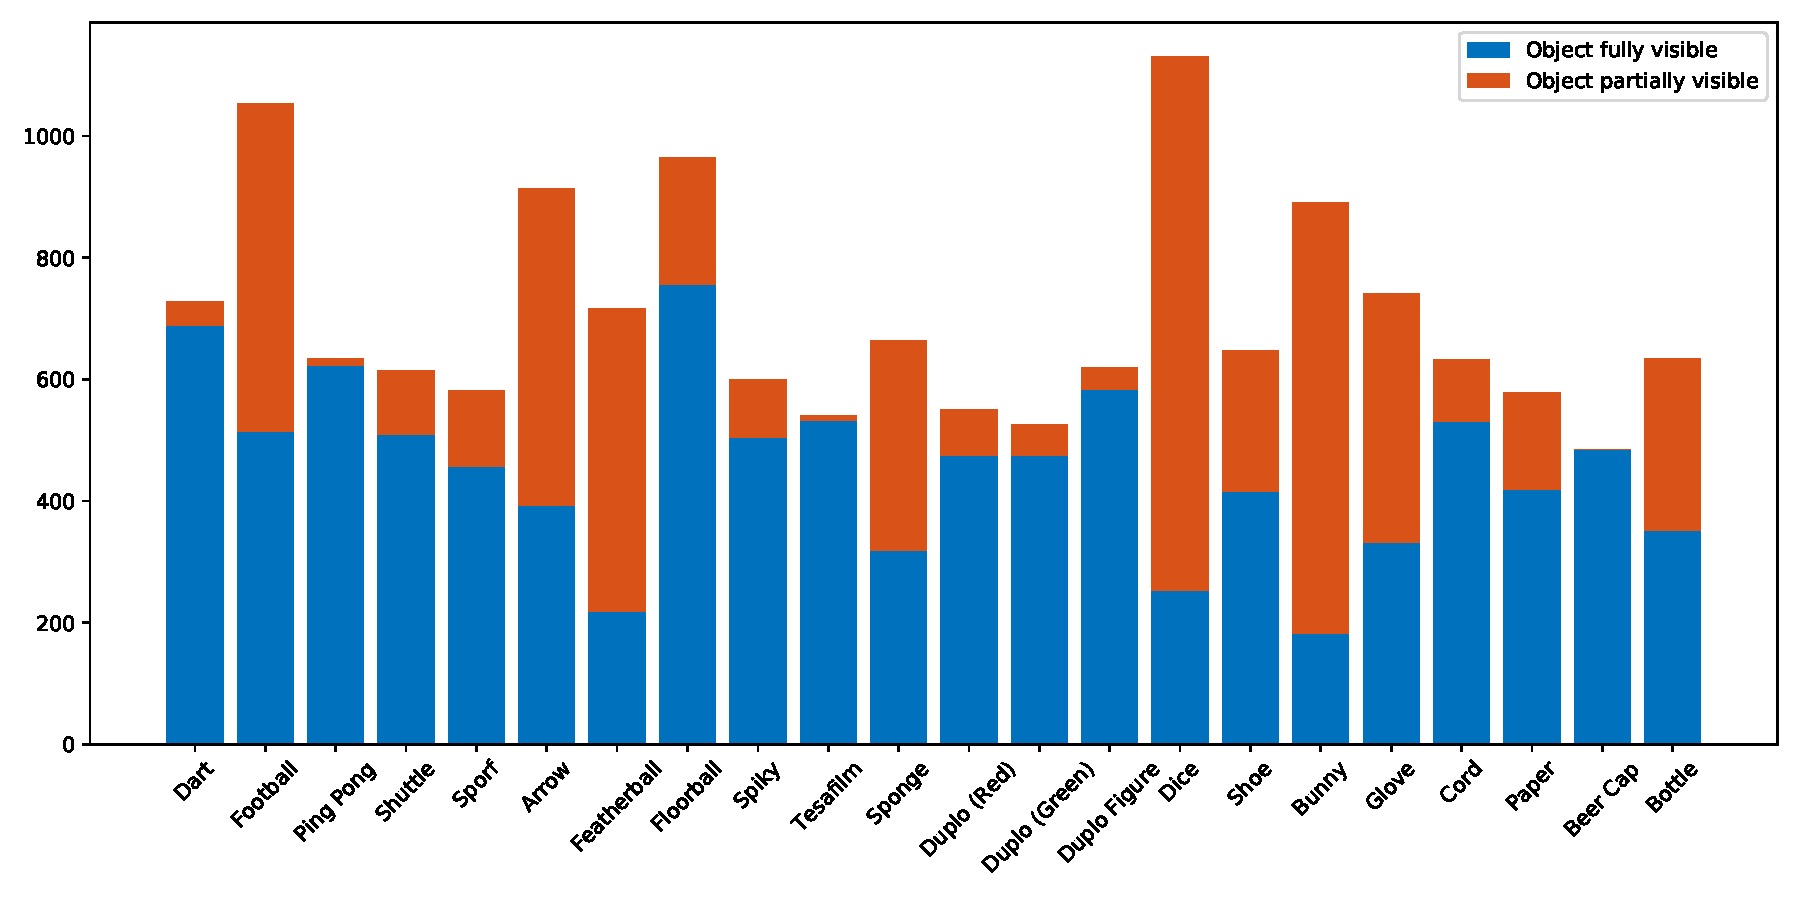
\includegraphics[width=\textwidth]{statistics}
  \caption{Statistics}
  \label{fig:statistics}
\end{figure}

\begin{figure}[h]
  \centering
  \begin{subfigure}[b]{0.45\textwidth}
    \centering
    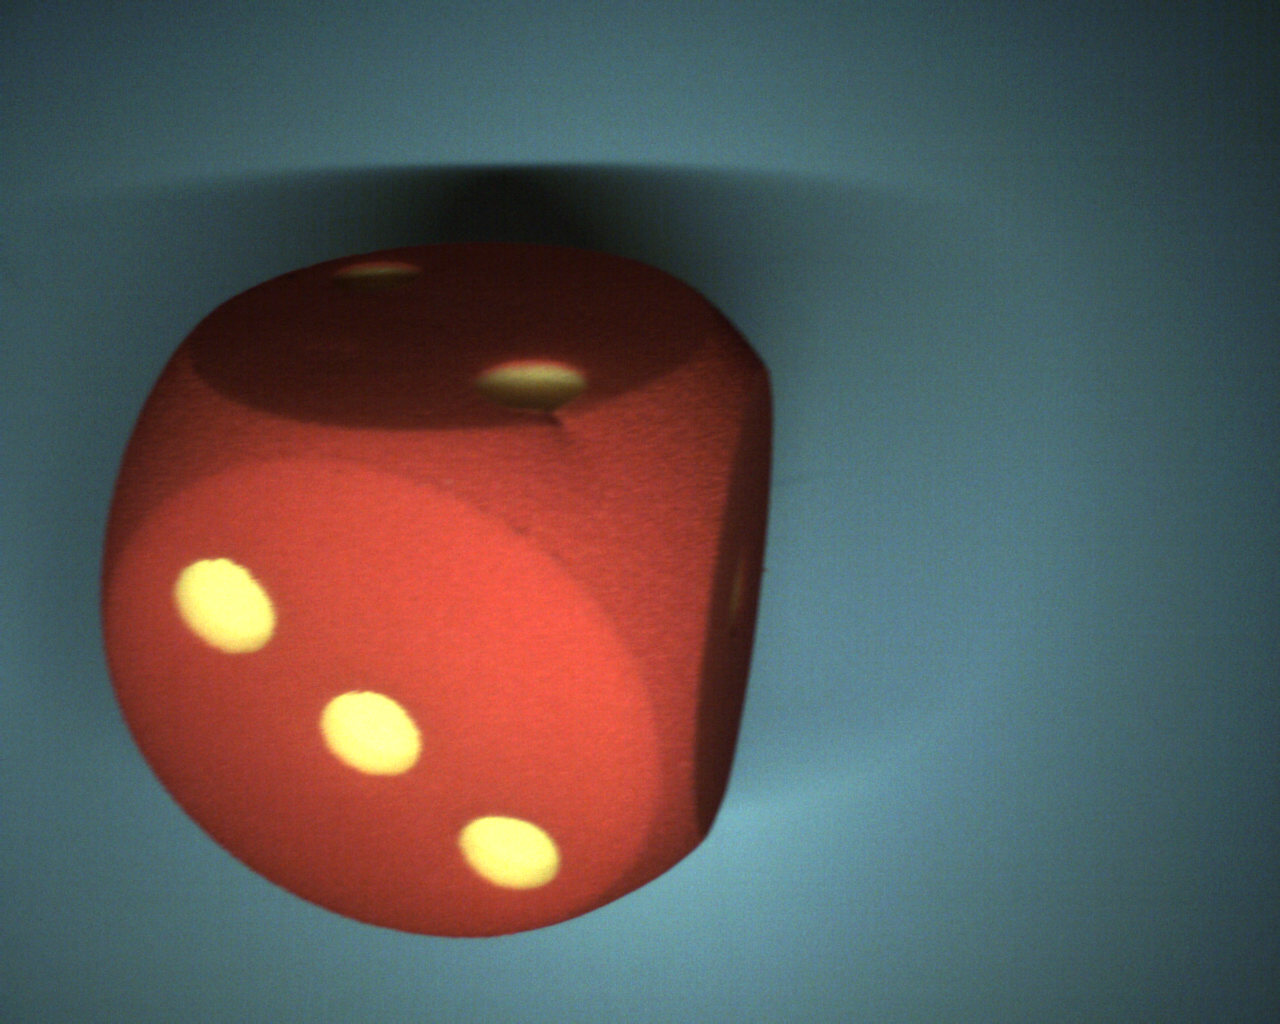
\includegraphics[width=0.9\textwidth]{1574950250_238_9_foam-dice}
    \caption{Continuous white balance}
    \label{subfig:foam_dice_first_day}
  \end{subfigure}
  \begin{subfigure}[b]{0.45\textwidth}
    \centering
    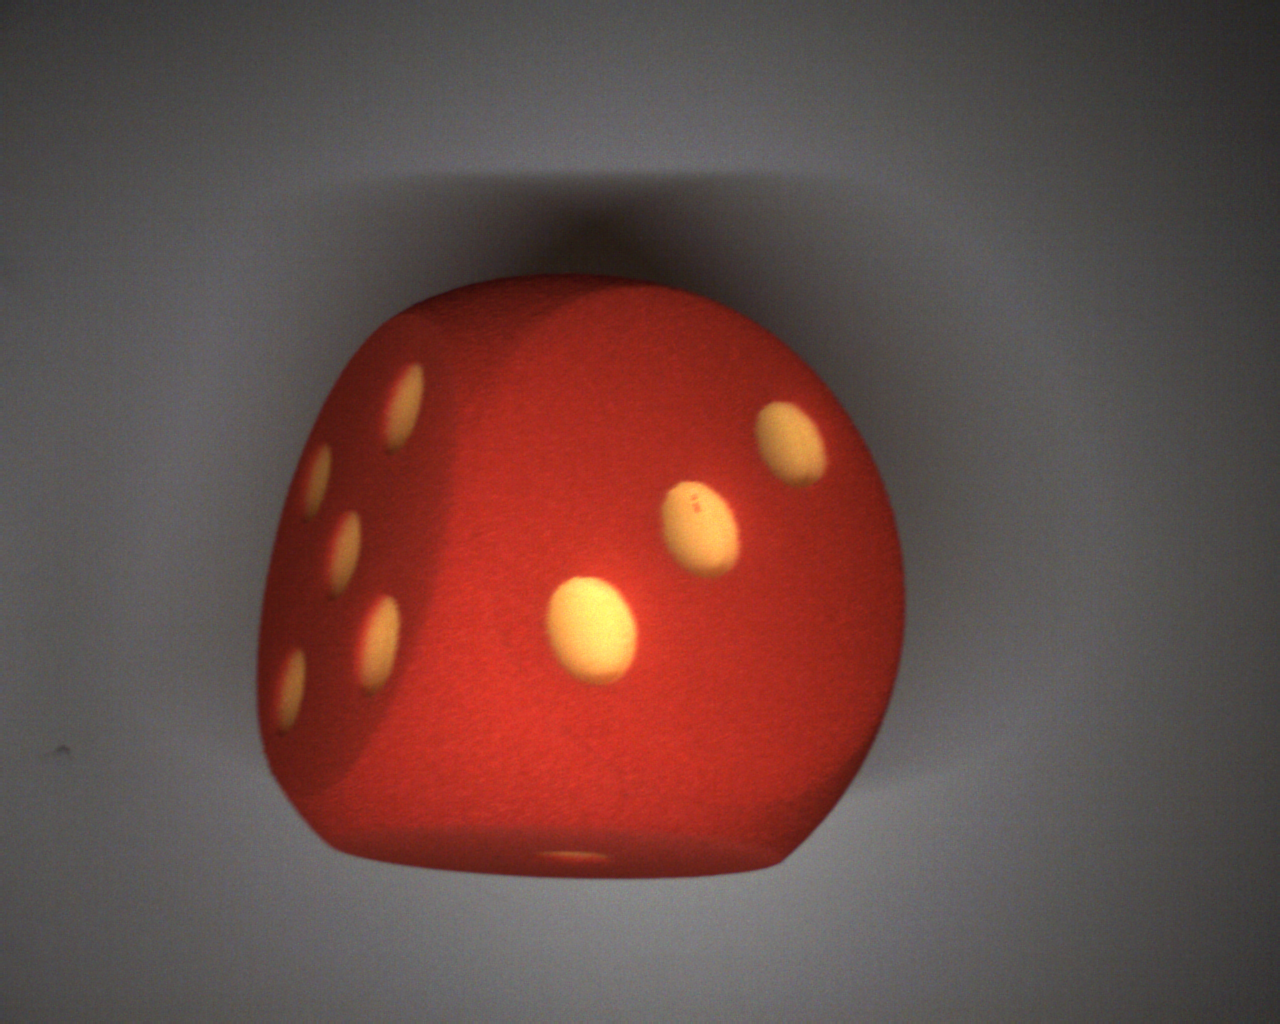
\includegraphics[width=0.9\textwidth]{1575032343_726_11_foam-dice}
    \caption{One-off white balance}
    \label{subfig:foam_dice_second_day}
  \end{subfigure}
  \caption{White balance difference between the first (\subref{subfig:foam_dice_first_day}) and the second (\subref{subfig:foam_dice_second_day}) day}
  \label{fig:dataset_white_balance}
\end{figure}

\section{Software}
\label{sec:software}

Collecting a sufficiently large dataset of pictures is not trivial.
% Why is it not trivial?
When done manually, the camera has to be started and stopped for each throw.
This likely creates many empty frames at the beginning and at the end of the capture.
Those empty and therefore invalid frames must be removed to avoid errors during the training of the CNN later on.
Furthermore, each valid frame must be labeled.
This procedure is very error-prone if it is performed manually for each individual frame.
% Solution
To simplify this task, a camera throw detection mechanism is implemented and various Python scripts are used.

This chapter describes the camera interface, the implemented throw detection mechanism, the used database and the various Python scripts.

\subsection{Camera Inteface}
\label{subsec:camera_interface}
% \todo[inline]{Chapter 'Camera Configuration' with all the settings at the end? Probably!}

Baumer provides the Baumer Generic Application Programming Interface (Baumer GAPI) to control its industrial cameras.
The Baumer GAPI supports the programming languages C\# and C++. For performance reasons C++ was used.

This section provides an overview of the Baumer GAPI, the available pixel formats and the camera connection interface USB3 Vision.

\subsubsection{Baumer GAPI Overview}
\label{subsubsec:baumer_gapi_overview}
% \todo[inline]{Citations}
% Baumer GAPI Programmers Guide (needs to be downloaded)

The Baumer GAPI is based on the Generic Interface for Cameras (GenICam).
It is a package of several libraries and the GenICam Producers (e.g. \texttt{bgapi2\_usb.cti}).
It provides the main classes that represent the logical and physical components of the image processing system.
Furthermore, it provides list classes to enable discovery and listing of the main objects.
There are even some additional classes to transform images and for debugging.
All classes are available through the namespace \texttt{BGAPI2} after including the header file \texttt{bgapi2\_genicam.hpp}.
% https://www.baumer.com/ch/en/product-overview/industrial-cameras-image-processing/software/baumer-gapi-sdk/c/14174

% https://www.baumer.com/ch/en/product-overview/industrial-cameras-image-processing/software/baumer-gapi-sdk/c/14174
\begin{table}[ht]
  \caption{Overview of the most important Baumer GAPI classes}
  \label{tab:baumer_gapi}
  \centering
  \begin{tabular}{llp{8.5cm}}
    \toprule
    \textbf{Main Classes} & \textbf{List Classes} & \textbf{Description} \\
    \midrule
     & \textbf{\texttt{SystemList}} & The class \texttt{SystemList} is used to discover objects of the class \texttt{System} (Producer). \\
    \midrule
    \textbf{\texttt{System}} & \textbf{\texttt{InterfaceList}} & The class \texttt{System} is the abstraction of the Producer and used to discover objects of the class \texttt{Interface}. \\
    \midrule
    \textbf{\texttt{Interface}} & \textbf{\texttt{DeviceList}} & The class \texttt{Interface} represents a physical interface (e.g. USB) and can be used to discover objects of the class \texttt{Device}. \\
    \midrule
    \textbf{\texttt{Device}} & \textbf{\texttt{DataStream}} & The class \texttt{Device} is used to configure the camera and can also be used to discover objects of the class \texttt{DataStream}. \\
    \midrule
    \textbf{\texttt{DataStream}} & \textbf{\texttt{BufferList}} & The class \texttt{DataStream} represents a data stream from the camera to the host and can be used to list objects of the class \texttt{Buffer}. \\
    \midrule
    \textbf{\texttt{Buffer}} &  & The \texttt{Buffer} class represents a single memory buffer and acts as the target for the image acquisition. \\
    \bottomrule
  \end{tabular}
\end{table}

\subsubsection{Pixel Formats}
\label{subsubsec:pixel_format}
% \todo[inline]{Citations, Document, that only 8bits are used? No.}
% (https://en.ids-imaging.com/tl_files/downloads/techtip/TechTip_18MP-color-sensor-as-mono_EN.pdf)

The Baumer industrial camera VCXU-13C uses the digital image sensor PYTHON1300 from ON Semiconductor and allows for the use of monochrome, raw and color pixel formats (see chapter \ref{sec:camera}).
The digital image sensor itself has 1280 $\times$ \SI{1024}{px} that aquire brightness with a bit depth of \SI{10}{bit}.
In order to capture color images, a color filter is applied to each individual pixel.
These red, green and blue (RGB or BGR) color filters only transmit light with a particular wavelength.
Due to the fact that the luminance perception of the human eye is most sensitive to green light, twice as many green filters are used as red and blue filters.
The color filters are arranged in a Bayer color matrix $B$, as shown in figure \ref{subfig:bayerrg} \cite{dcs}.

There are several modifications of the Bayer pattern that can be achieved by simply shifiting the pixels around.
The pattern in figure \ref{subfig:bayergr} is achieved by shifting the initial pattern one pixel to the left, whereas the pattern in figure \ref{subfig:bayergb} is achieved by shifting the pattern one pixel up.

The different Bayer patterns are usually named after the color of the elements $B_{1,1}$, $B_{1,2}$, $B_{2,1}$ and $B_{2,2}$.
This results in the four possible patterns \texttt{RGGB}, \texttt{GRBG}, \texttt{GBRG} and \texttt{BGGR}.

However, there exist different naming conventions for the different Bayer patterns.
Baumer labels the Bayer patterns after the color of the elements $B_{1,1}$ and $B_{1,2}$, resulting in the name \texttt{BayerRG} for figure \ref{subfig:bayerrg}.
The Open Computer Vision Library (OpenCV) labels them after the elements $B_{2,2}$ and $B_{2,3}$, resulting in the name \texttt{BayerBG} for the same figure \ref{subfig:bayerrg} \cite{baumer_opencv}.

In order to create an RGB color image from the raw Bayer pattern image, a demosaicing (also ``debayering'') algorithm is necessary.
The Baumer industrial camera VCXU-13C is able to transform the raw sensor data into the respective RGB or BGR values in real time.
Another possibility is to do the required color space transformation with the OpenCV function \texttt{cv::cvtColor}.
Since OpenCV uses the BGR instead of the standard RGB color space, the required color space conversion code is \texttt{cv::COLOR\_BayerBG2BGR}.
This will convert the raw Bayer pattern image into a BGR image \cite{opencv_csc}.

\begin{figure}[ht]
  \centering
  \begin{subfigure}[b]{0.3\textwidth}
    \centering
    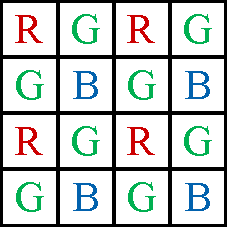
\includegraphics[scale=1]{bayerrg}
    \caption{\texttt{RGGB} (Baumer \texttt{BayerRG})}
    \label{subfig:bayerrg}
  \end{subfigure}
  \begin{subfigure}[b]{0.3\textwidth}
    \centering
    
\includegraphics[scale=1]{bayergr}
    \caption{\texttt{GRBG} (Baumer \texttt{BayerGR})}
    \label{subfig:bayergr}
  \end{subfigure}
  \begin{subfigure}[b]{0.3\textwidth}
    \centering
    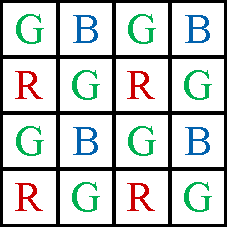
\includegraphics[scale=1]{bayergb}
    \caption{\texttt{GBRG} (Baumer \texttt{BayerGB})}
    \label{subfig:bayergb}
  \end{subfigure}
  \caption{Bayer color matrices $B$}
  \label{fig:bayer}
\end{figure}

\clearpage
\subsubsection{USB3 Vision Interface}
\label{subsubsec:usb3_vision_interface}
\todo[inline]{Citations, Colon after caption of tables?, Table H instead of h}

The Baumer industrial camera VCXU-13C uses the USB3 Vision (U3V) interface with a maximum transfer rate of \SI{5}{Gbit/s} $\approx$ \SI{596}{MiB}.
The max. frame rate is \SI{222}{fps} and the total pixel count is equal to
\[
\text{Pixel}_\text{tot} = \text{Pixel}_\text{width} \cdot \text{Pixel}_\text{height} = \SI{1280}{px} \cdot \SI{1024}{px} = \SI{1310720}{px}.
\]

To calculate the required data rate in bytes per second, equation \ref{eq:data_rate} can be used.

\begin{equation}
  \text{Req. data rate} = \text{Pixel}_\text{tot} \cdot \text{Byte per pixel} \cdot \text{Frame rate}
  \label{eq:data_rate}
\end{equation}

For this application a fixed frame rate of \SI{200}{fps} is sufficient and facilitates the calculations.

Table \ref{tab:data_rates} shows the required data rates for the Baumer pixel format \texttt{BayerRG8} and \texttt{BGR8}.
It is evident that due to the maximum transfer rate of \SI{596}{MiB} of the U3V interface, only the Baumer \texttt{BayerRG8} pixel format is suitable.
% https://www.baumer.com/ch/de/produktubersicht/industriekameras-bildverarbeitung/industriekameras/cx-serie/usb-3-0-schnittstelle/vcxu-13c/p/23792

\begin{table}[h]
  \caption{Required data rate for the two Baumer pixel formats \texttt{BayerRG8} and \texttt{BGR8}}
  \label{tab:data_rates}
  \centering
  \begin{tabular}{lll}
    \toprule
     & \textbf{\texttt{BayerRG8}} & \textbf{\texttt{BGR8}} \\
    \midrule
    \textbf{Bytes per pixel} & \SI{1}{B} & \SI{3}{B} \\
    \textbf{Frame rate} & \SI{200}{fps} & \SI{200}{fps} \\
    \textbf{Req. data rate} & \SI{250}{MiB/s} & \SI{750}{MiB/s} \\
    \bottomrule
  \end{tabular}
\end{table}

% \subsubsection{Camera Configuration}
\label{subsubsec:camera_configuration}
% \todo[inline]{}

The camera configuration should be the same during data collection and deployment.
For this reason, the optimal parameters have been carefully selected.
Table \ref{tab:config} lists the important configurations and their respective values.

\begin{table}[hb]
  \caption{Camera configuration}
  \label{tab:config}
  \centering
  \begin{tabular}{lll}
    \toprule
    \textbf{Parameter} & \textbf{Value} & \textbf{Description} \\
    \midrule
    BalanceWhiteAuto & \texttt{Once} & Perform the white balance once during setup \\
    Gain & 4 & For the max. brightness, the max. gain is used \\
    ExposureTime & \SI{250}{\micro\second} & A short exposure time of \SI{250}{\micro\second} is used \\
    AcquisitionFrameRateEnable & \texttt{true} & Enable fixed frame rate \\
    AcquisitionFrameRate & \SI{200}{fps} & Set fixed frame rate to \SI{200}{fps} \\
    TriggerMode & \texttt{Off} & Use no trigger (free run) \\
    PixelFormat & \texttt{BayerRG8} & Use the raw Baumer \texttt{BayerRG8} pixel format \\
    \bottomrule
  \end{tabular}
\end{table}

\clearpage

\subsection{Throw Detection Mechanism}
\label{subsec:throw_detection_mechanism}

To reliably detect a throw, a simple image change detection algorithm is implemented.
It requires a repeated difference computation and therefore a circular buffer is used.

% This section explains the algorithm with its required components and the saving of the images.
This section explains the employed algorithm, its implementation and the saving of the images.

% \subsubsection{Image Change Detection Algorithm}
% \subsubsection{Throw Detection Algorithm}
\subsubsection{Employed Algorithm}
\label{subsubsec:algorithm}
% \todo[inline]{No citations?! Or OpenCV?! Or Baumer?!}

% image change detection algorithm vs throw detection / throw detection mechanism / throw detection algorithm => throw detection employs icda

% Goal of the throw detection is to extract the valid frames of a throw from the continous data stream
  % valid frames have object on them, invalid frames are empty (background)
% real-time
% serial process, 200 fps => >5 ms to process each frame
% not a lot of time for a complex (fancy) algorithm => simplest one possible is used
  % for the throw detection algorithm a simple image change detection algorithm is used

% Algo: computation of the difference and comparison to a threshold to detect changes in the picture

% what this sections describes

% Due to the in section {} mentioned bandwidth limitations of the U3V interface the raw bayer is processed
  % conversion to BGR8 takes too long! => use raw bayer for the detection
% Saving images takes time + unnecessary => saving at the end!
  % see section \ref

% buffers

% frame_id (FID) to keep track of ...
% uses 2 flags and 2 "pointers" to the buffer

% compared against threshold (if mean_diff < threshold, considered to be no change [equal sign])

% throw begin and throw end, what happens

% Why are the last two frames are not valid?
  % only possible to detect the end when there is no change any longer

The goal of the throw detection is to extract valid frames of a throw --- with objects on them --- from the continous data stream of the camera.
Therefore, the throw detection needs to work in real time.
At a frame rate of \SI{200}{fps}, there is $<\SI{5}{ms}$ to process a single frame (without the use of parallel computing).
Due to this time constraint, a simple image change detection algorithm is employed.

\paragraph{Image Change Detection Algorithm}
\vspace{-20pt}
\begin{enumerate}
  \item Compute the absolute difference between the current and the last frame
  \item Compute the average among all the pixels of the difference
  \item Compare the mean difference against a threshold value
\end{enumerate}

This section describes how the throw detection works.
The complete listing of the throw detection can be found in appendix \ref{app:throw_detection}.
The implementation of the image change detection is described in section \ref{subsubsec:image_change_detection}.
Furthermore, the way the threshold value is obtained is documented in section \ref{subsubsec:threshold}.

Due to the bandwidth limitations of the U3V interface mentioned in section \ref{subsubsec:usb3_vision_interface}, the received images are in the raw Bayer pixel format.
A conversion from the Baumer \texttt{BayerRG8} to \texttt{BGR8} takes too long an therefore the raw frames are processed.
Moreover, the valid images are only saved on the hard disk at the end of a throw, as this also takes a lot of time (see section \ref{subsubsec:saving_images}).

For the above reasons, two image buffers are used.
The received images are stored in Baumer \texttt{BGAPI2::Buffer} objects.
To save the images later on, a circular buffer for OpenCV matrices (\texttt{cv::Mat}) is used.
This is documented in section \ref{subsubsec:buffers}.
The size of those image buffers (\texttt{BS}) determines the max. amount of valid frames $N_\text{max}$ that can be captured.

To keep track of the present and past frames, a frame id (\texttt{FID}) is utilized.
Furthermore, two flags are used to mark the beginning and the end of a throw.

Whenever the mean difference between two consecutive frames is greater than or equal to the threshold, they are considered to be different ($\ne$).
Otherwise, the two frames are considered to be equal ($=$).

Once two consecutive frames are different, the flag \texttt{throw\_bgn} is set to \texttt{true} and the current \texttt{FID} is saved in \texttt{throw\_bgn\_idx}.
The current and all subsequent frames --- except for the last two --- belong to the detected throw until two consecutive frames are no longer different.
In this case, the flag \texttt{throw\_end} is set to \texttt{true} and the current \texttt{FID} is saved in \texttt{throw\_end\_idx}.

The last two frames are not valid due to the way the throw detection works.
The first invalid frame occurs when the object leaves the image, as this is still a change in the image and thus not detected.
The second invalid frame results from the fact that the following images are only now the same and therefore the current \texttt{FID} is saved.

Figure \ref{subfig:algorithm_general_case} shows the general case of the just described throw detection.
As already mentioned, the max. amount of valid frames $N_\text{max}$ depends on the image buffer size (\texttt{BS}).
To properly detected a throw, the amount of valid frames $N$ must meet the condition
\[
  N \in \{1..(\text{BS}-2)\}.
\]
In the current implementation, an image buffer size of \SI{1000}{} is used and therefore $N_\text{max} = \SI{998}{frames}$.
An example of three valid frames ($N = 3$) is shown in figure \ref{subfig:algorithm_example_3}.

\begin{figure}[h]
  \centering
  \begin{subfigure}[b]{\textwidth}
    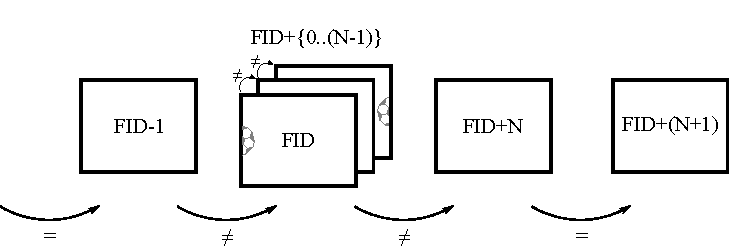
\includegraphics[scale=0.85]{algorithm}
    \caption{General case with $N \in \{1..(\text{BS}-2)\}$}
    \label{subfig:algorithm_general_case}
  \end{subfigure}
  \begin{subfigure}[b]{\textwidth}
    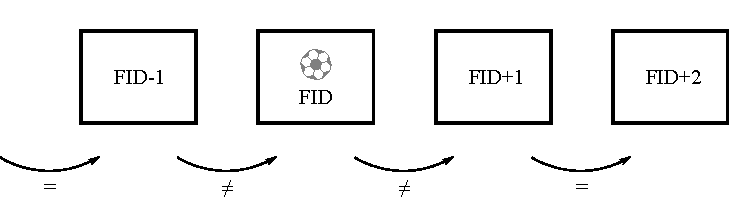
\includegraphics[scale=0.85]{algorithm_ex_1}
    \caption{Example of $N_\text{min} = 1$}
    \label{subfig:algorithm_example_1}
  \end{subfigure}
  \begin{subfigure}[b]{\textwidth}
    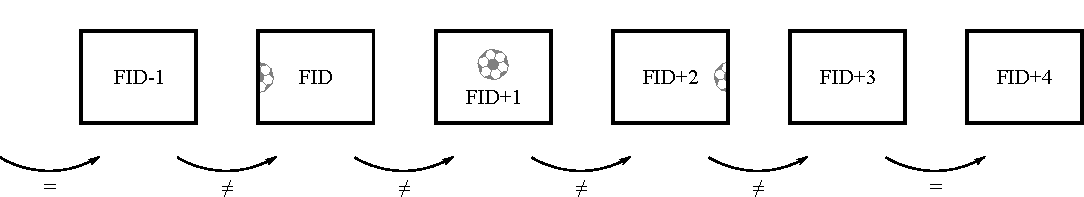
\includegraphics[scale=0.85]{algorithm_ex_3}
    \caption{Example of three valid frames ($N = 3$)}
    \label{subfig:algorithm_example_3}
  \end{subfigure}
  \caption{Illustration of the throw detection}
  \label{fig:throw_detection}
\end{figure}

\subsubsection{Baumer Image Buffer}
\label{subsubsec:baumer_buffer}
% \todo[inline]{Citations}

% Buffer handling by Baumer => large buffer sizes (here not a problem), could be handled by ourselves!
  % handle this by ourselves on the Ultra96 board, due to memory size constrains

\subsubsection{OpenCV Circular Buffer}
\label{subsubsec:opencv_buffer}
% \todo[inline]{Citations}

% OpenCV \texttt{Mat}

% opencv matrix circular buffer (same size as Baumer buffer but shallow [shallow-copy])
  % only pointer to the baumer pixel data
  % copying would require a lot of space and time (which is not much to play with), thus main reason time
% circular buffer graphic

\begin{lstlisting}[style=C++]
  cv_buffer[frame_id % buff_size] = cv::Mat(height, width, CV_8UC1, (void *) pBufferFilled->GetMemPtr());
\end{lstlisting}

\subsubsection{Difference Computation}
\label{subsubsec:difference_computation}
% \todo[inline]{Citations, Picture of how the diff. is calculated or matrices?}

% computation of the difference how it is done with opencv

% done for every frame except the first one (FID = 0)

% after the threshold averaging (see chapter threshold) ?!

\begin{lstlisting}[style=C++]
  cv::absdiff(cv_buffer[frame_id % buff_size], cv_buffer[(frame_id - 1) % buff_size], cv_abs);
  mean_diff = cv::sum(cv_abs)[0] / (width * height);
\end{lstlisting}

\subsubsection{Threshold Value Determination}
\label{subsubsec:threshold}
% \todo[inline]{Citations, Nico is this correct (regarding the 50 Hz flicker)?}

% how is the Threshold Value Determination done:
% average difference to obtain threshold (with pictures)
    % => 50 Hz flicker reduction

\begin{figure}[H]
  \centering
  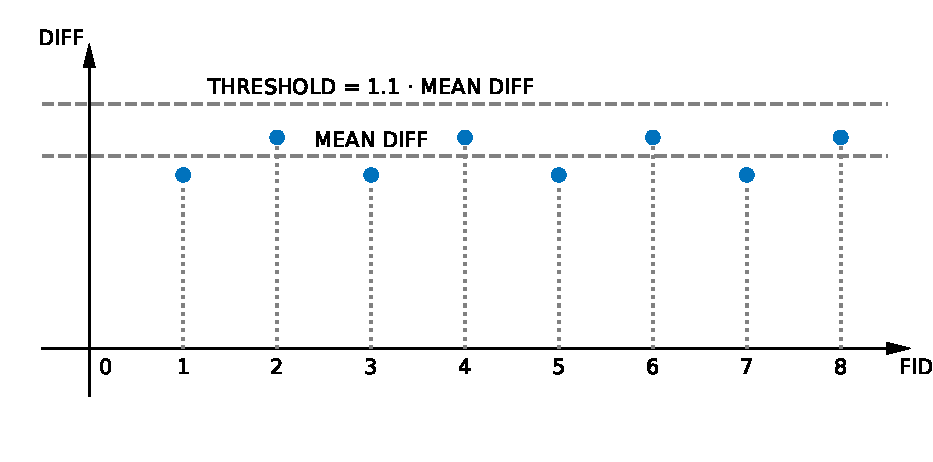
\includegraphics[width=0.75\textwidth]{threshold}
  \caption{Derivation of the threshold value from eigth averaged differences} % 
  \label{fig:threshold}
\end{figure}

\subsubsection{Saving Images}
\label{subsubsec:saving_images}
% \todo[inline]{Citations, Why PNG and not BMP or JPG?}

Resulting in the file names `\texttt{$\{0..(N-1)\}$.png}' (with $N$ beeing the amount of valid frames).

\begin{lstlisting}[style=C++]
  for (int i = throw_bgn_idx; i < (throw_end_idx - 1); ++i) {
    cv::cvtColor(cv_buffer[i % buff_size], cv_transformed, cv::COLOR_BayerBG2BGR);
    cv::imwrite(output_path + std::to_string(i - throw_bgn_idx) + ".png", cv_transformed);
  }
\end{lstlisting}

% https://www.baumer.com/ch/en/service-support/know-how/technical-information-industrial-cameras/baumer-gapi-and-opencv/a/baumer-gapi-and-opencv


\subsection{Database}
\label{subsec:database}

% why using a DB, since the picture names contain all the info already (easy of use in scripts)
% MySQL DB description with column names and data types

All images contain their respective labels in the file name.
% This is useful when manually looking through them but not optimal for a program.
This is useful for manually going through them, but not optimal for a program.
% The program would have to list all files and crawl through the file names.
The program would have to crawl the directory containing the images and parse the file names.
% This requires operations that involve the file system which are usually very slow.
This requires file system related operations, which are usually very slow.
The solution is to use a database that is designed to read and write such data.
% For this reason, a \textit{MySQL} database is used to store the labels and the file names.
For this reason, a MySQL database is used to store the labels, file names and other metadata.
Table \ref{tab:tab_frames_structure} lists all columns of the database table \texttt{aionfpga.frames}.

\begin{table}[hb]
  \caption{Structure of the database table \texttt{aionfpga.frames}}
  \label{tab:tab_frames_structure}
  \centering
  \begin{tabular}{llll}
    \toprule
    \textbf{Column} & \textbf{Type} & \textbf{Length} & \textbf{Description} \\
    \midrule
    id & \texttt{INT} &  & Sequence number (unique identifier) \\
    timestamp & \texttt{INT} &  & The Unix timestamp at the time of the throw \\
    throwid & \texttt{INT} &  & Throw sequence number \\
    frameid & \texttt{INT} &  & Frame sequence number within a throw \\
    frame & \texttt{VARCHAR} & 255 & The file name of the frame \\
    object & \texttt{VARCHAR} & 255 & The name of the object in the frame (label) \\
    framegood & \texttt{INT} &  & \texttt{0}: frame unusable | \texttt{1}: frame usable \\
    partial & \texttt{INT} &  & \texttt{0}: object fully visible | \texttt{1}: object partially visible \\
    \bottomrule
  \end{tabular}
\end{table}

\clearpage
\subsection{Python Scripts}
\label{subsec:python_scripts}

% creation of the data acquisition and alteration (daa) module with settings and definitions (functions)
% short summary of the function of each python script


\section{Experiences}
\label{sec:experiences}

The FHNW still has very little experience in the field of artificial intelligence on an FPGA.
Therefore the first part of the project was only about collecting information.
Due to the fact that Xilinx hardware was given research could be focused on this product.
Aside from the hardware definition the field of AI was still a very big world, fairly unknown to us.
With the help of Youtube, other internet research and books we slowly worked our way into the unknown zone. 
With time the topic became more accessible to us, but there were still questions to which we have no right answers yet.
For example how good must the picture quality be? 
May pictures be used if the object is only partially in the picture?
How many pictures per object are enough?
Questions which are normally answered by experience.
From our lack of experience we have marked cut-off images in the database, kept the quality as high as possible and informed ourselves about the sizes of other data sets on the Internet.

We also learned the hard way when choosing a camera with too little experience.
The plug and play version of a webcam sounded attractive, but turned out to be useless for moving objects.

The Python scripts turned out to be a reasonable investment.
If we had started and stopped all throws with the Baumer application, countless empty images would have to be removed before and after the throw.
Thanks to the real-time image comparison we saved this work.
The additional effort for configuring the camera via script also benefits us in project 6.

At the end of this project, the results can be seen.
We are in possession of a litter stand, a data set with more than \num{15000} images, as well as knowledge about AI.

\section{Thesis Prospect}
\label{sec:thesis_prospect}
% BOX fabrication / net -- 
% CNN -- The CNN model is developed and trained in Python 3 using TensorFlow 2 and the images collected in project 5.
% parallel change detection algo.
% High-Performance Implementation --  The advantages of an FPGA flow into the development. Thus, special attention is paid to the performance of the system.
% OS / application
% Verification -- The accuracy and performance of the CNN model implemented on the FPGA is verified.

This project will be continued as a thesis in the next semester.
The throwing booth will be upgraded with the Fibox and a net construction.
The box can be manufactured according to the finished drawings, but the net construction has to be drawn first.
The net holder will most likely be manufactured with a 3D printer.

The CNN model is developed and trained in Python 3 using TensorFlow 2 with the dataset collected during this project.
%In order to be able to evaluate the changes of the images on the ARM, a parallelization will probably be necessary.
In order to be able to use the throw detection mechanism on the quad-core ARM-based processor, parallel computing will probably be necessary.
The reason for this is the lower clock speed of the ARM Cortex-A53 processors for the same amount of data.

As soon as this is realized, the next step is to implement the trained CNN model on the FPGA.
With sufficient time resources, an additional focus can be placed on speed optimizations.

At the same time a Linux-based operating system (OS) is put into operation on the MPSoC.
The application shows the recognized object to the user at the trade fair.
This function is implemented on the ARM Cortex-A53 as well.

To measure the quality of the developed system, the accuracy of the convolutional neural network is evaluated.
Special attention is paid to the differences between the implementation on the computer and the implementation on the embedded system.


% Bibliography
\printbibliography[heading=bibintoc]
\label{sec:literature}
\clearpage

% Glossary
%\printglossaries
%\clearpage

% Appendix
\begin{appendix} \todo{Drawings noch korrekt einfügen, sind nur mal drinn, um verweisen zu können.}
  \section{Problem Statement}
  \label{app:problem_statement}
  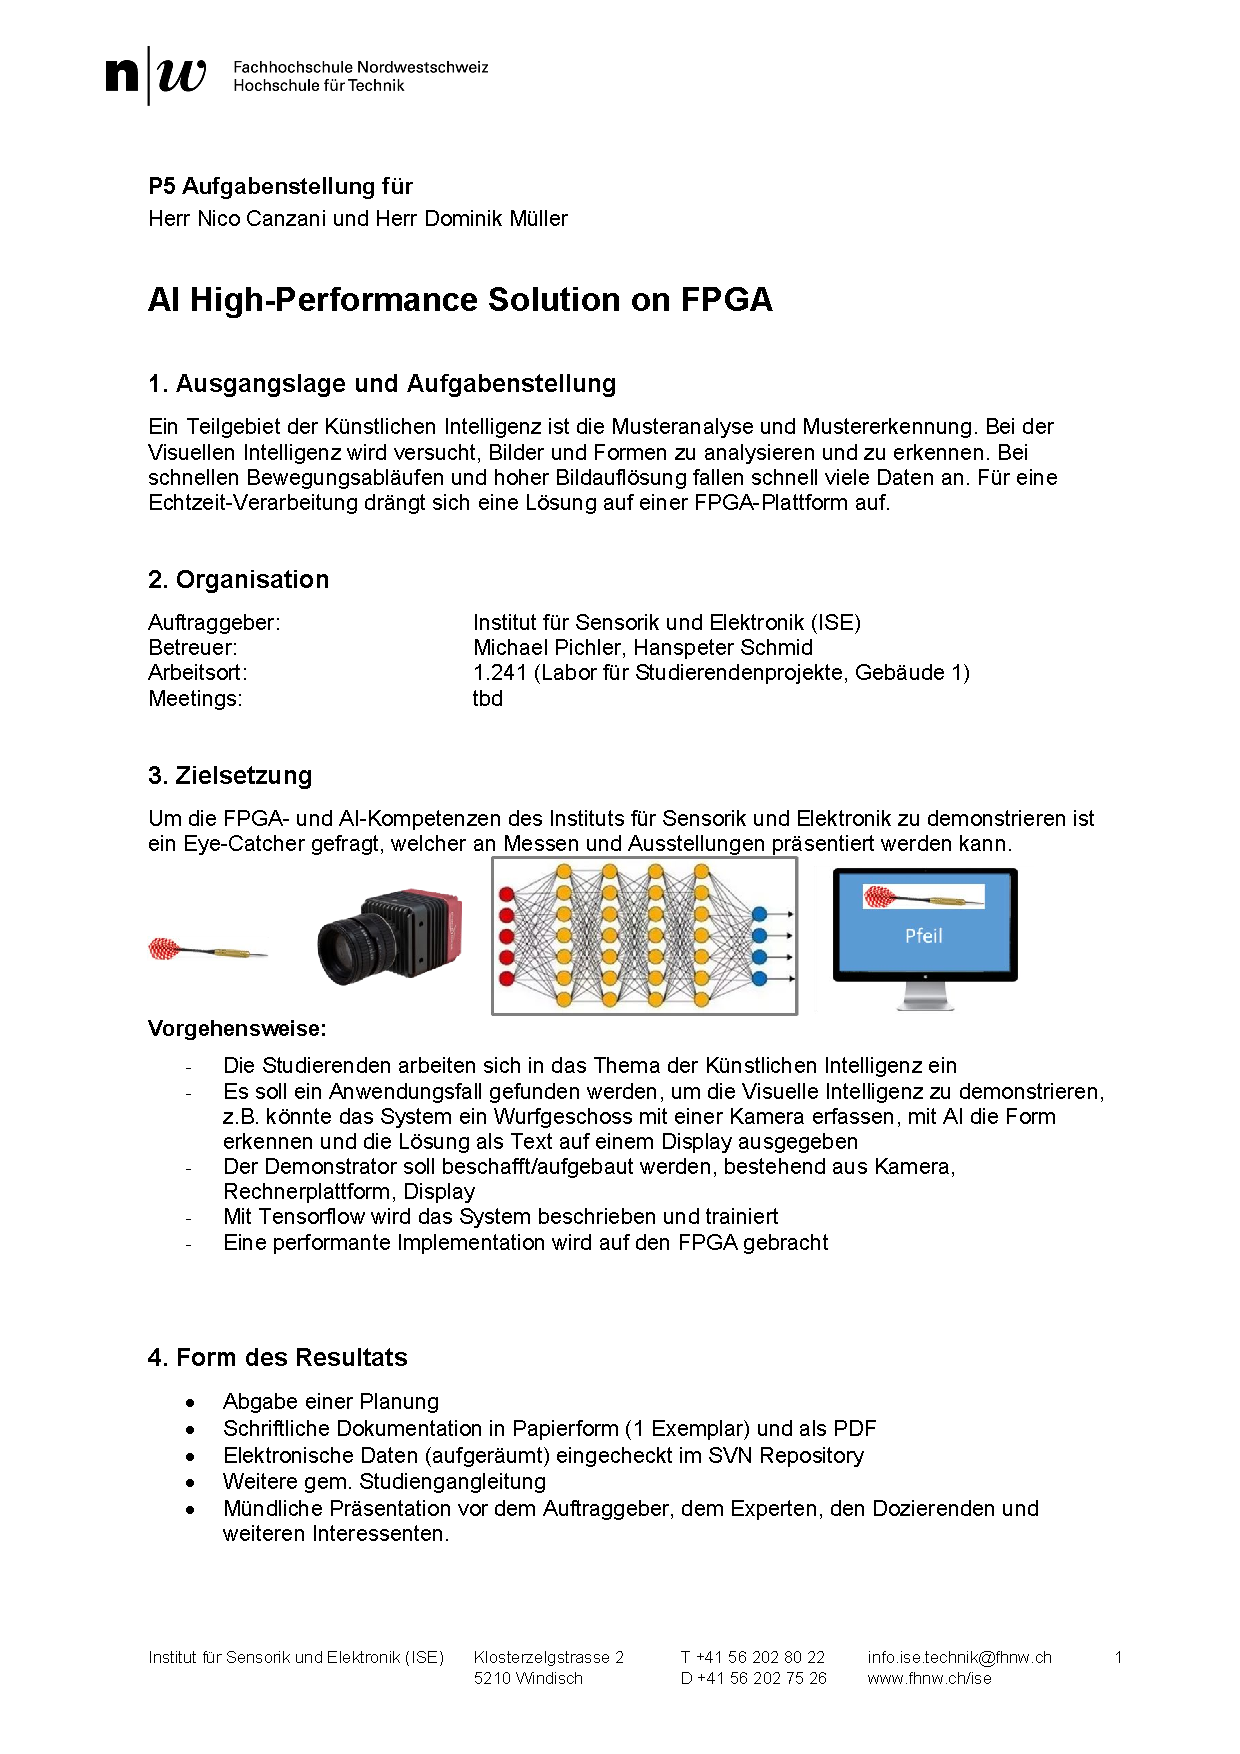
\includepdf[pages=-]{appendix/problem_statement.pdf}
  % 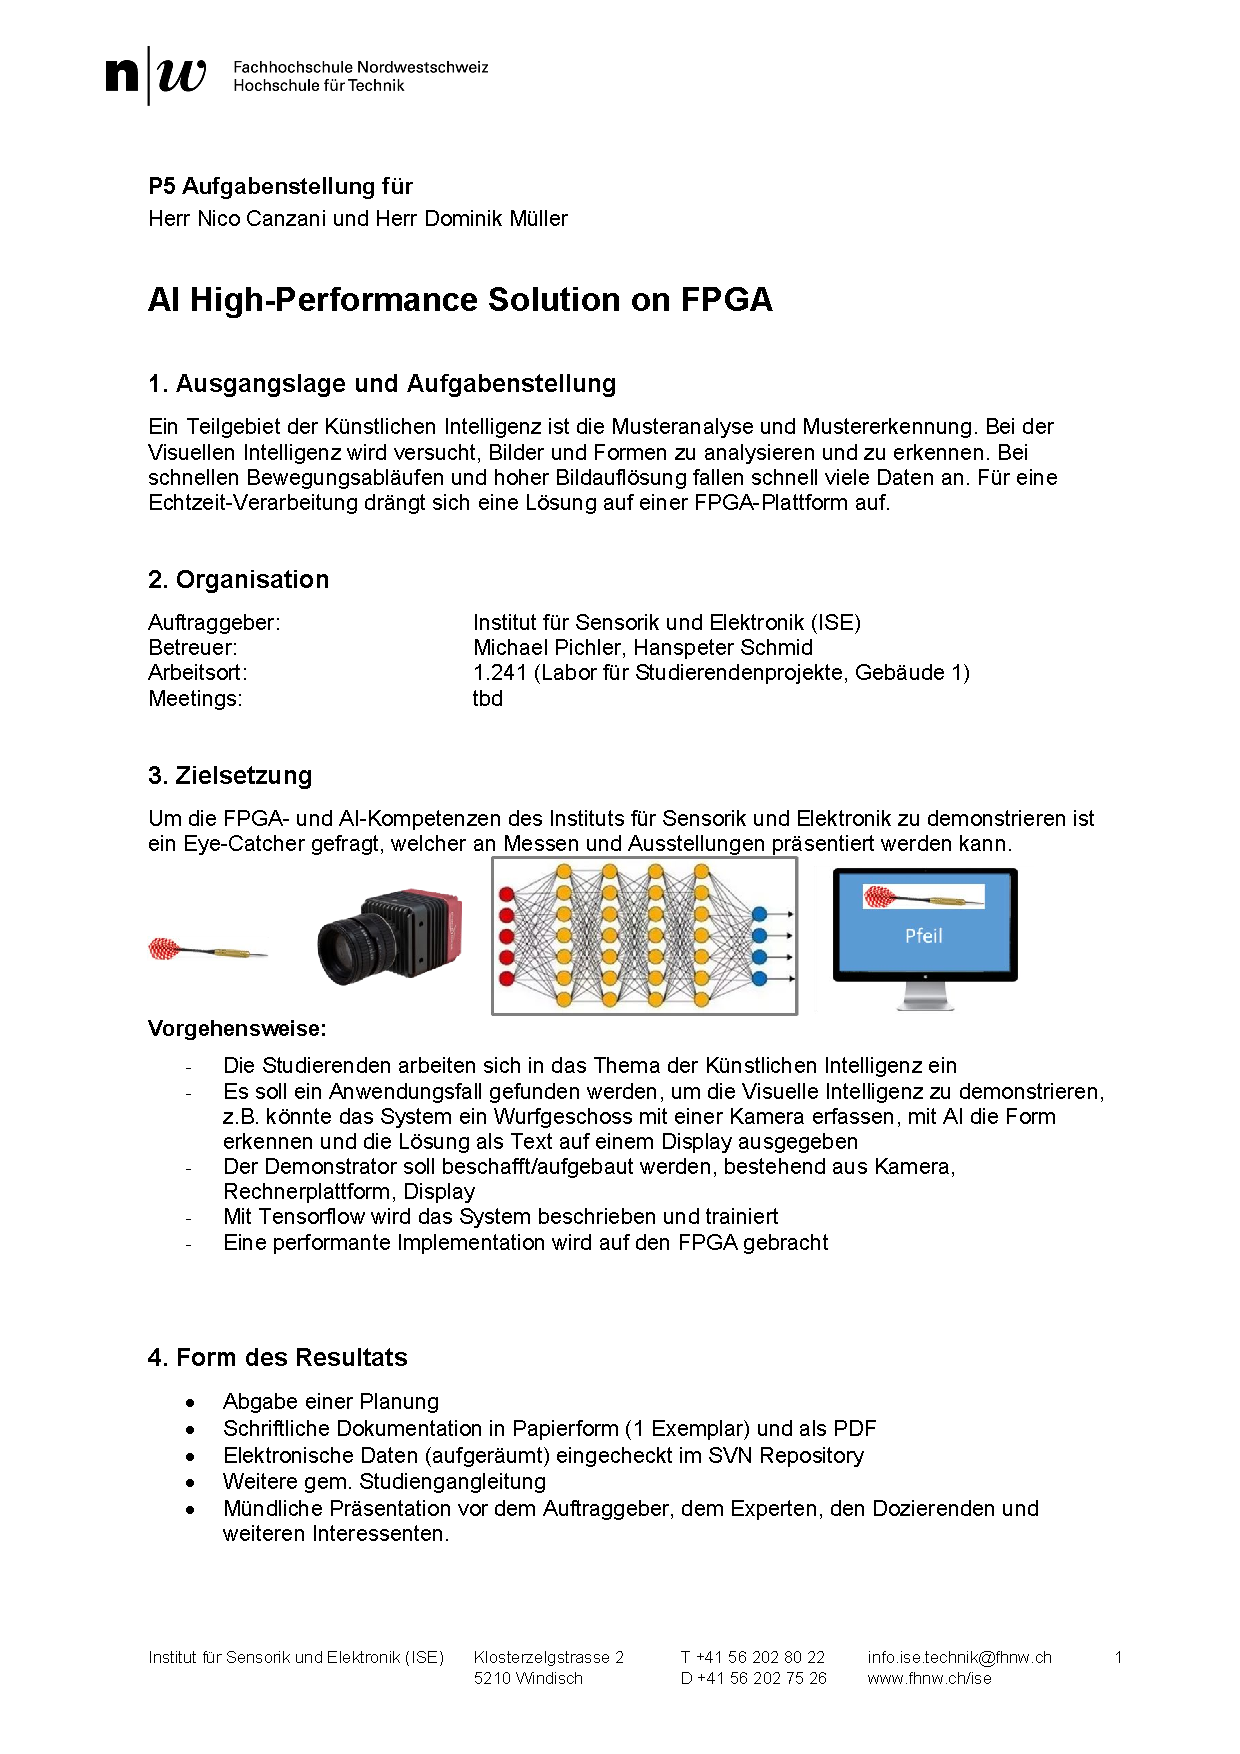
\includepdf[pages=-,nup=1x2,landscape=true]{appendix/problem_statement.pdf}

  \section{Drawing Camera Protection}
  \label{app:drawings_camera_protection}
  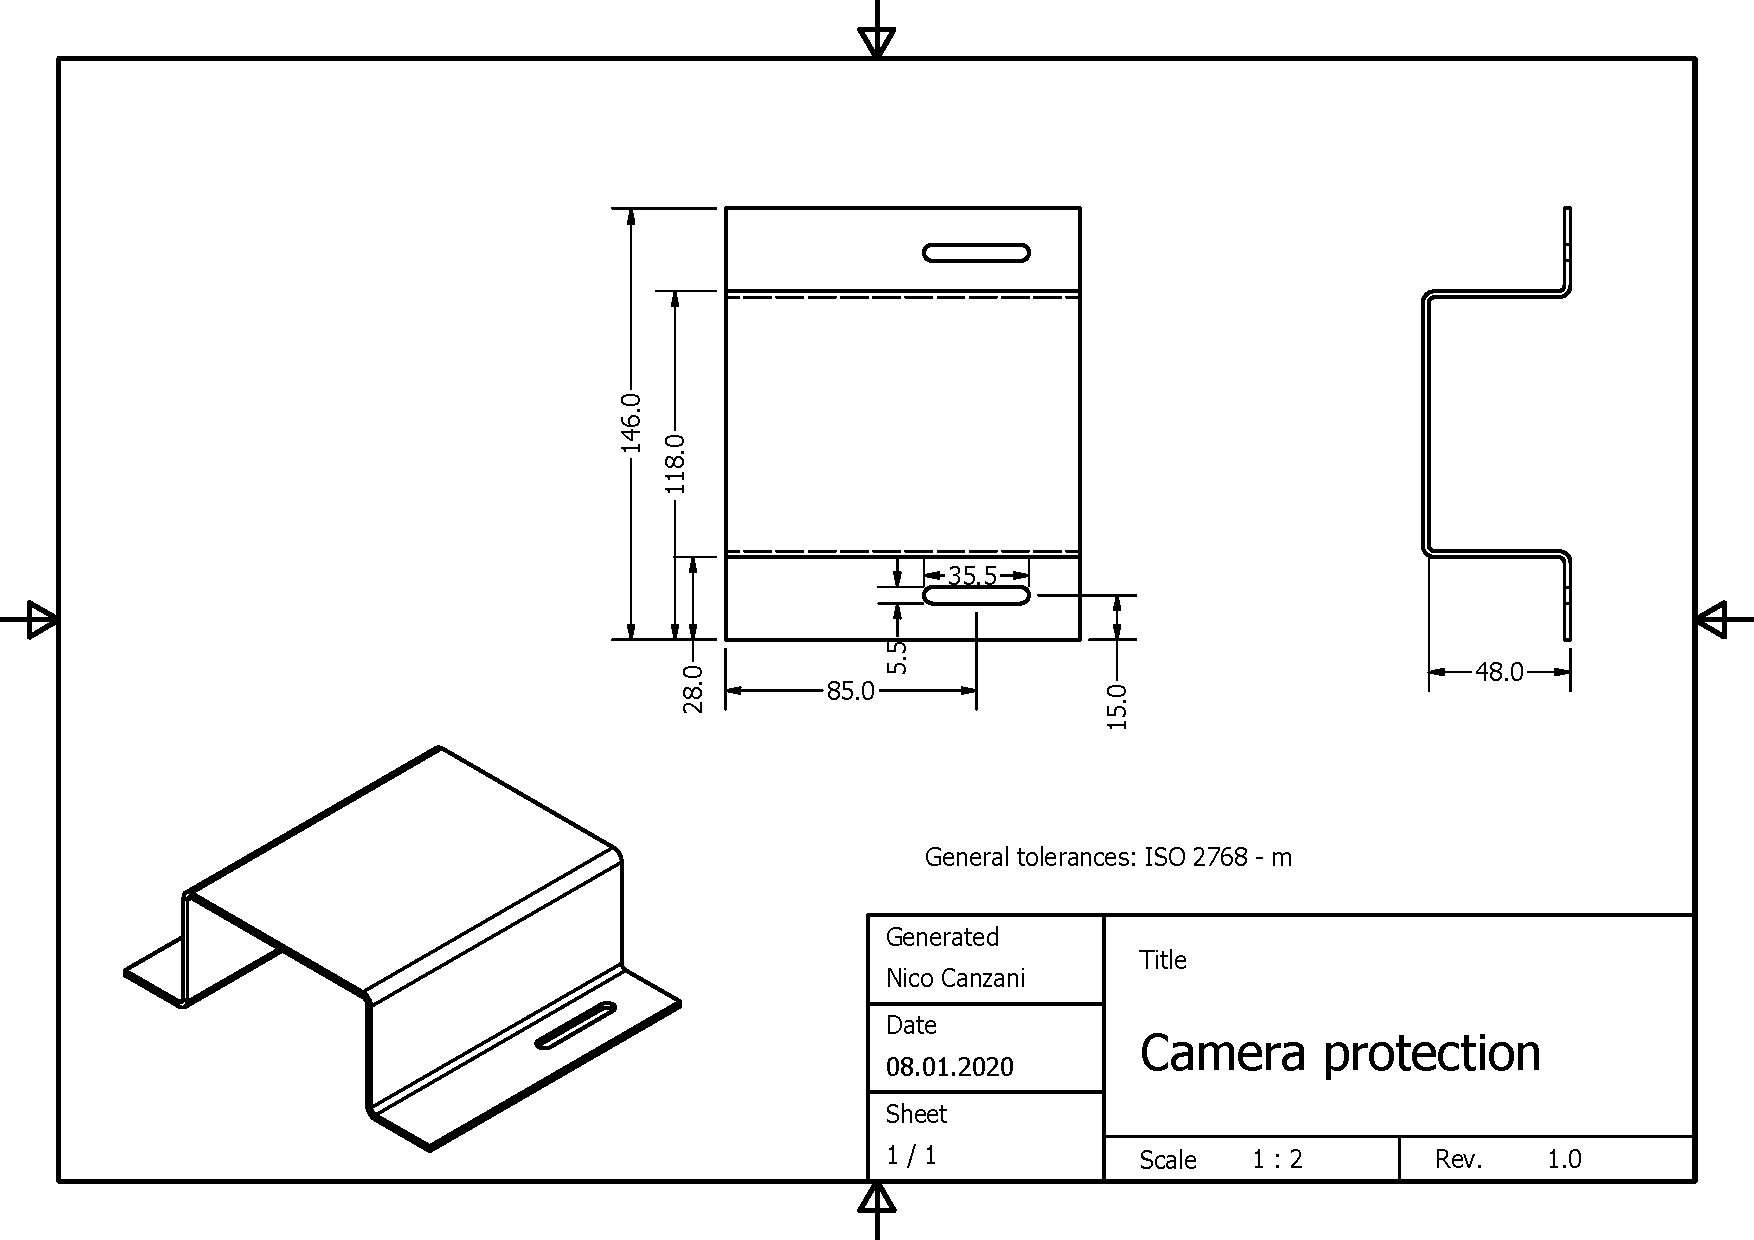
\includepdf[pages=-,landscape=true]{appendix/drawings_camera_protection.pdf}

  \section{Drawing Fibox}
  \label{app:drawings_fibox_bottom}
  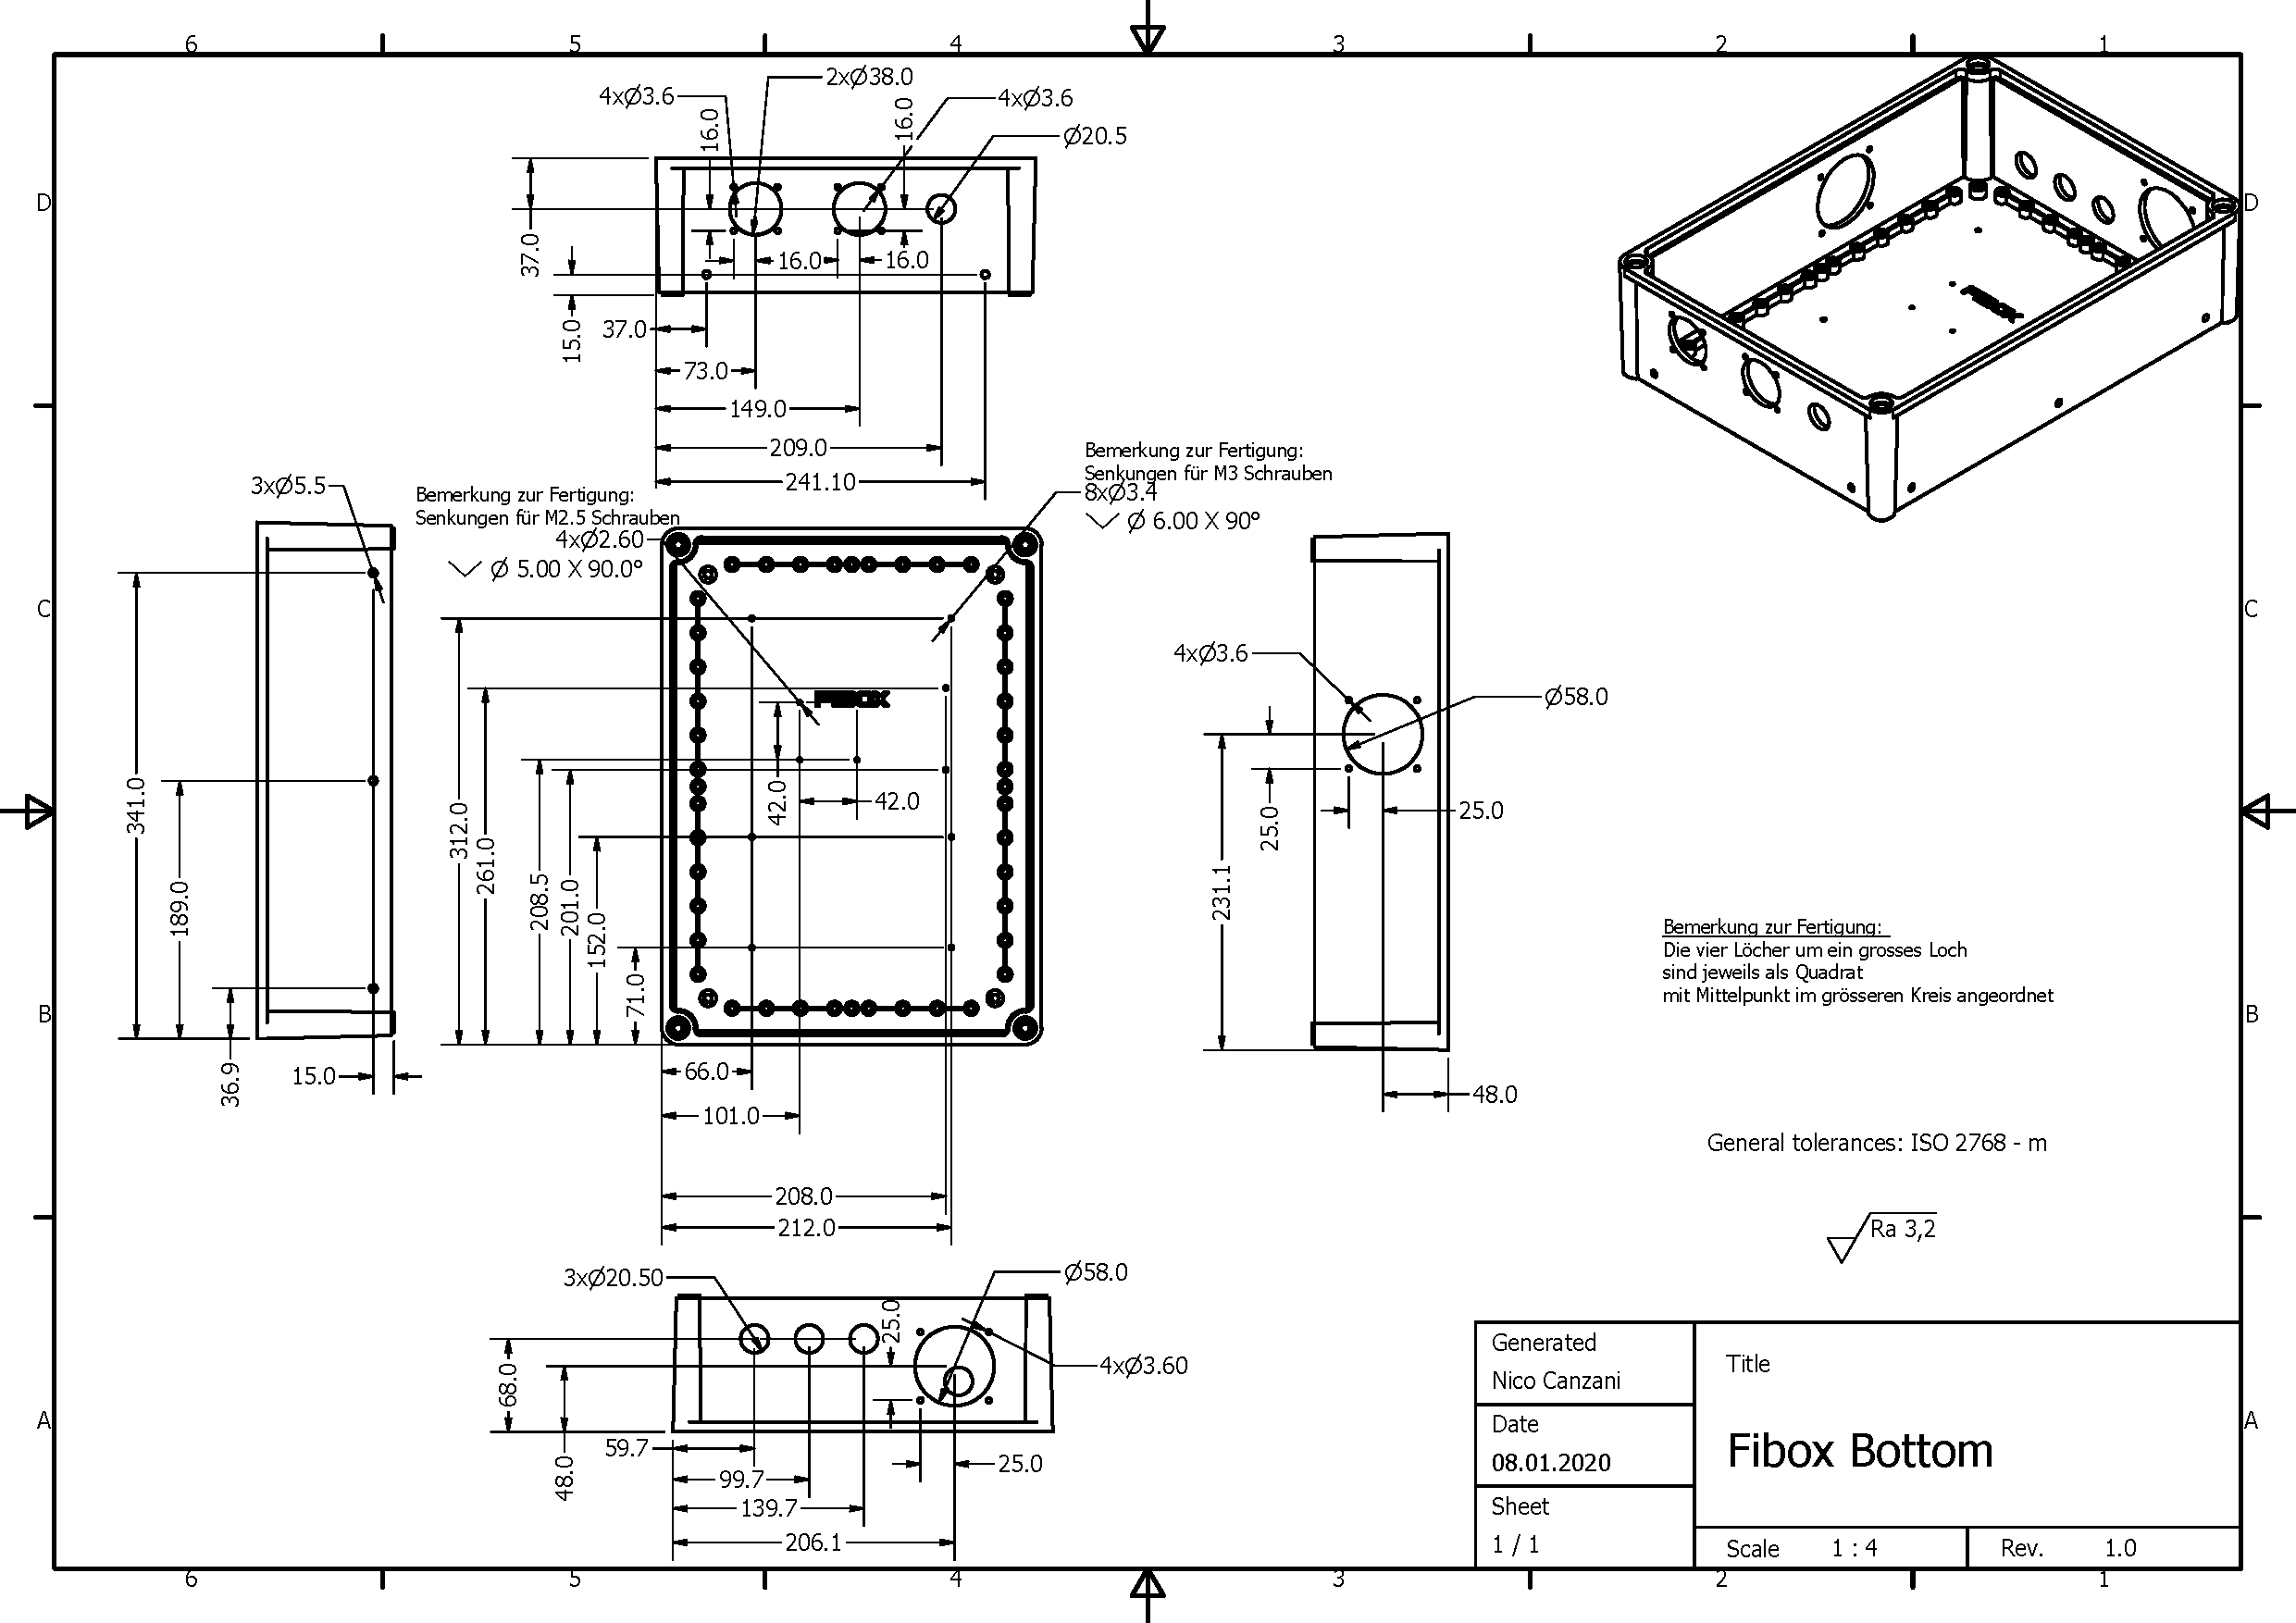
\includepdf[pages=-,landscape=true]{appendix/drawings_fibox_bottom.pdf}

  \section{Drawing Mounting Adapter}
  \label{app:drawings_mounting_adapter}
  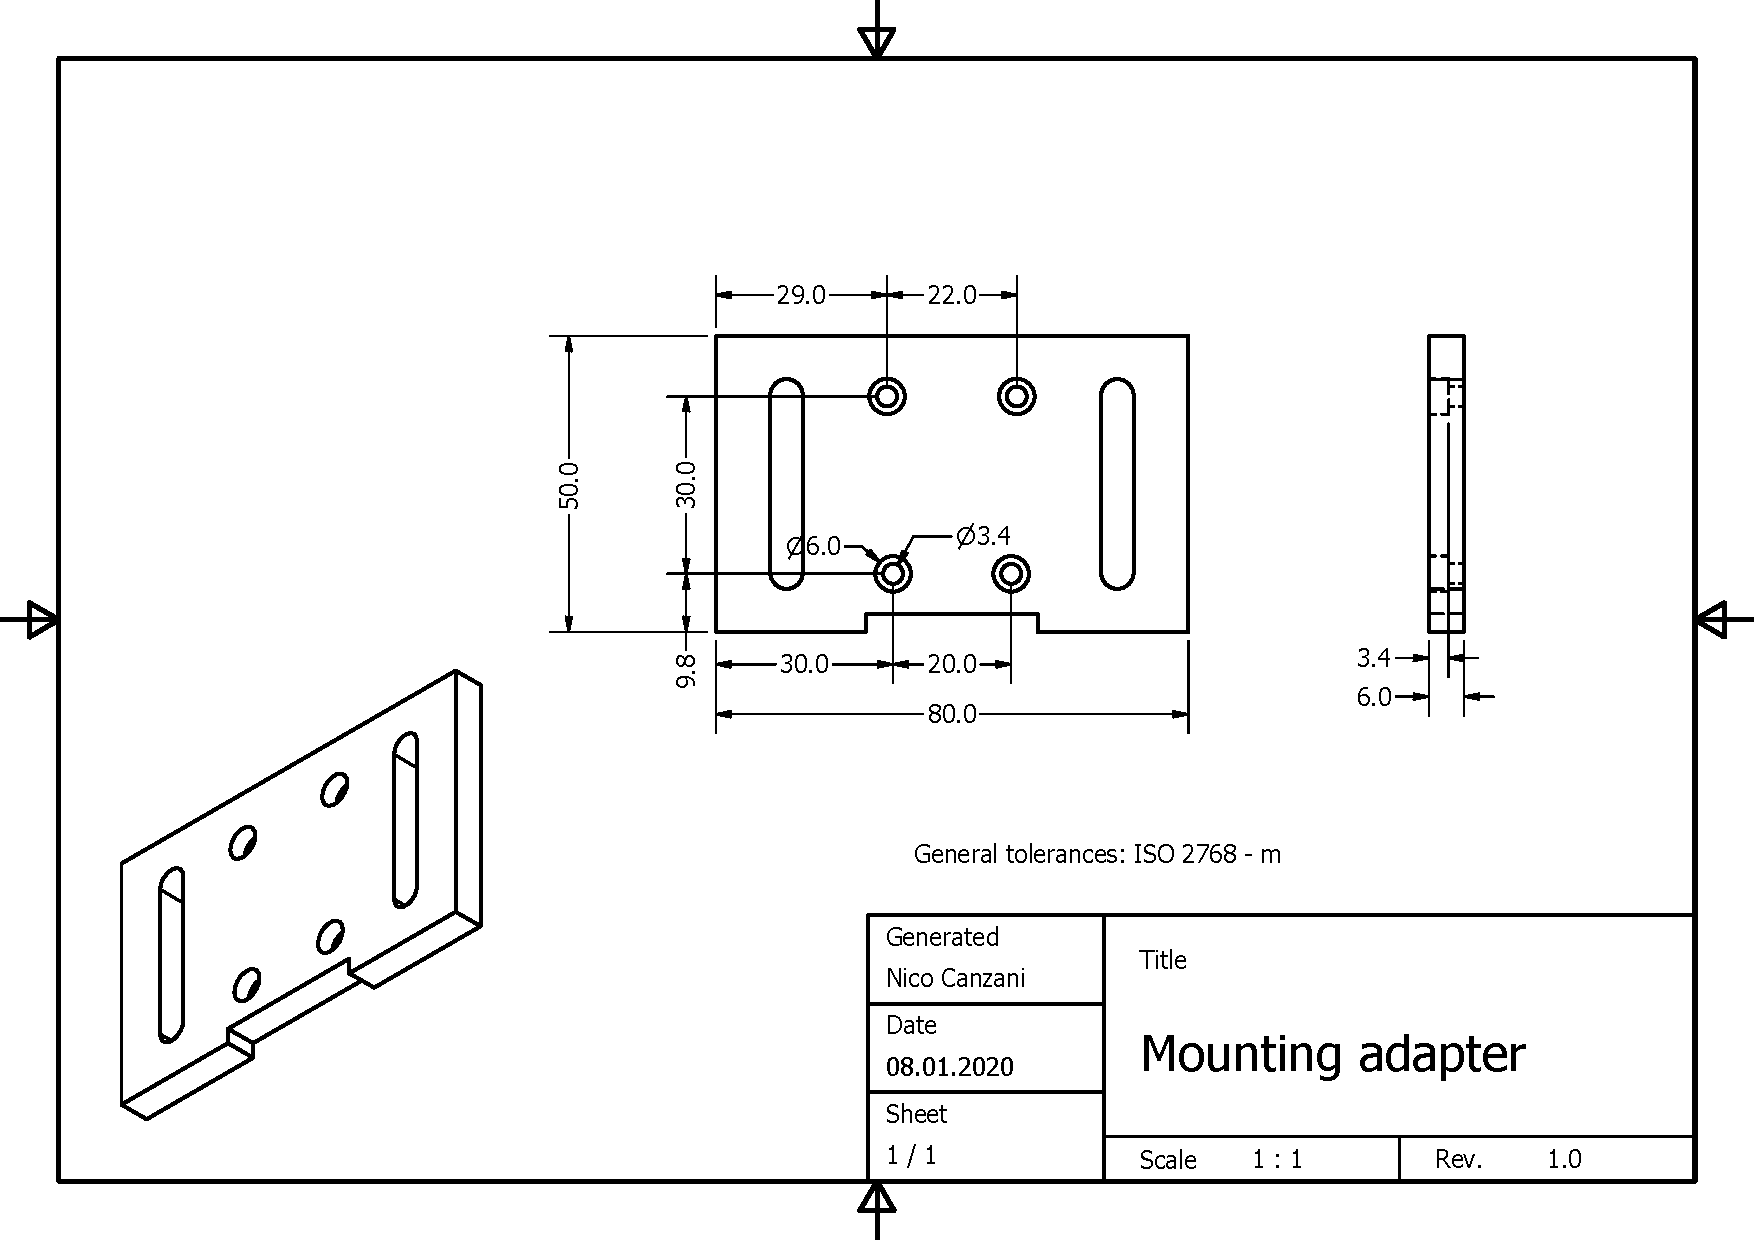
\includepdf[pages=-,landscape=true]{appendix/drawings_mounting_adapter.pdf}

  \section{Drawing Rear Panel}
  \label{app:drawings_rear_panel}
  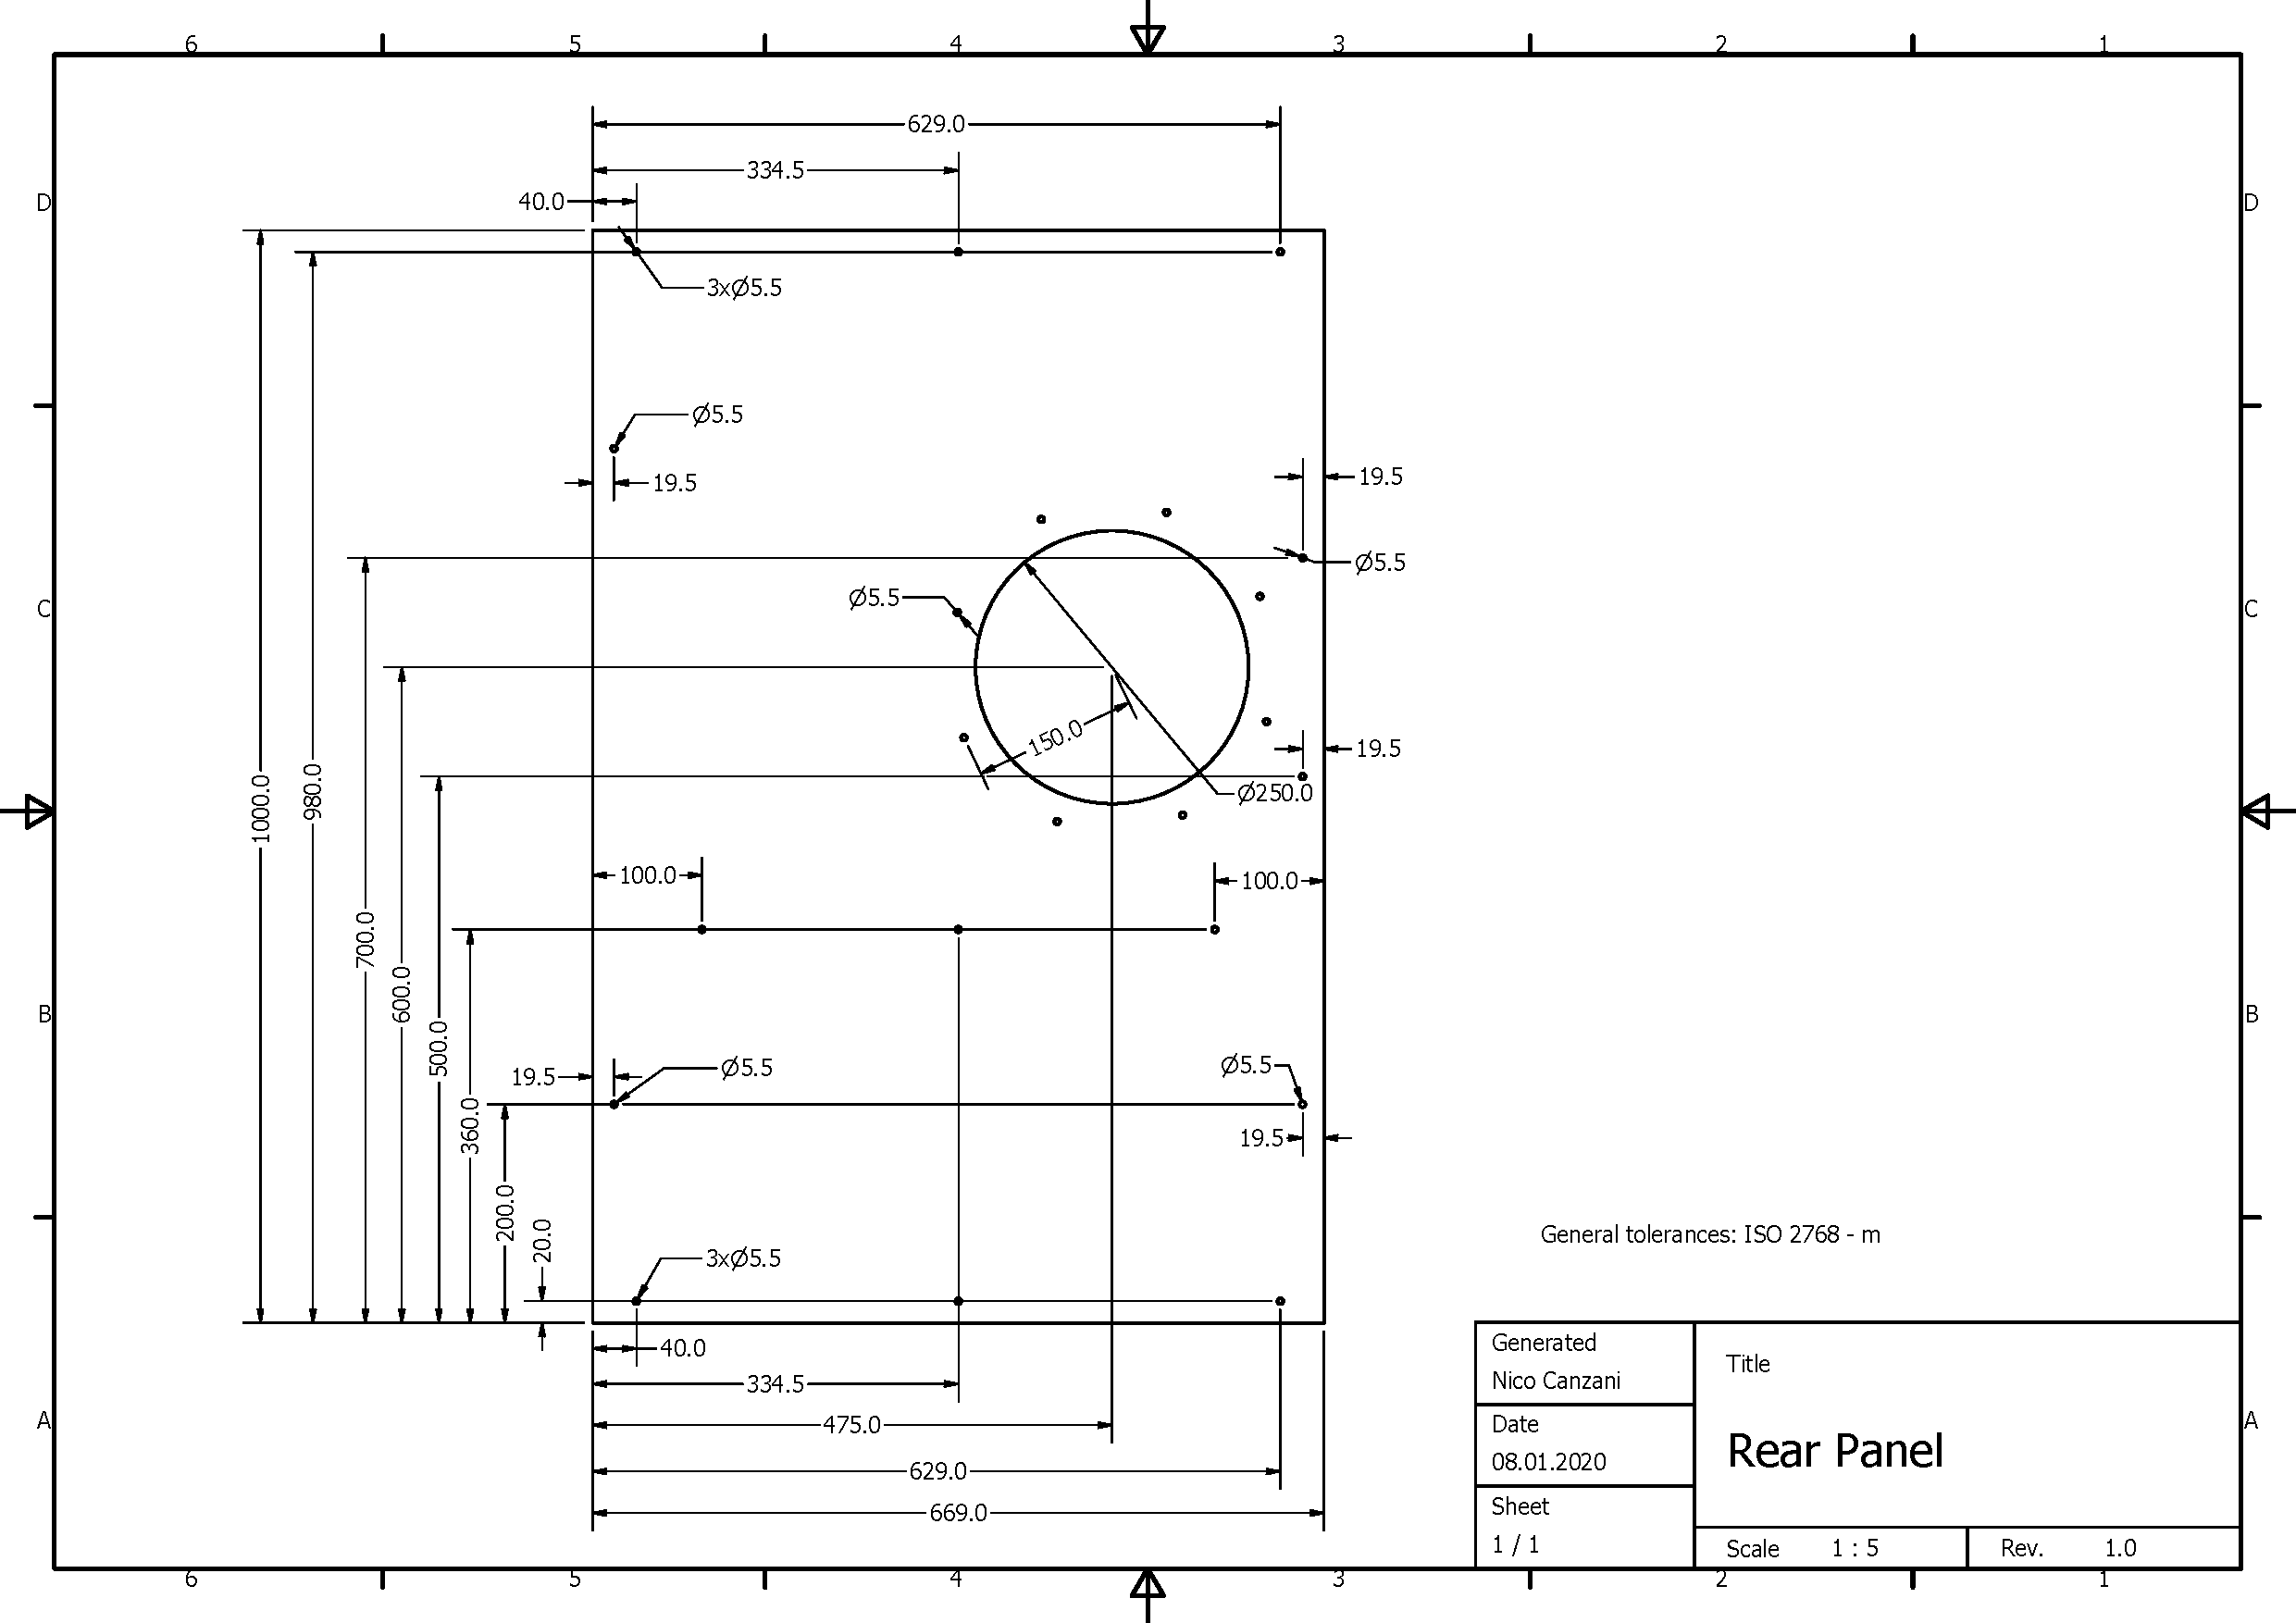
\includepdf[pages=-,landscape=true]{appendix/drawings_rear_panel.pdf}

  \section{Drawing Side Panel}
  \label{app:drawings_side_panel}
  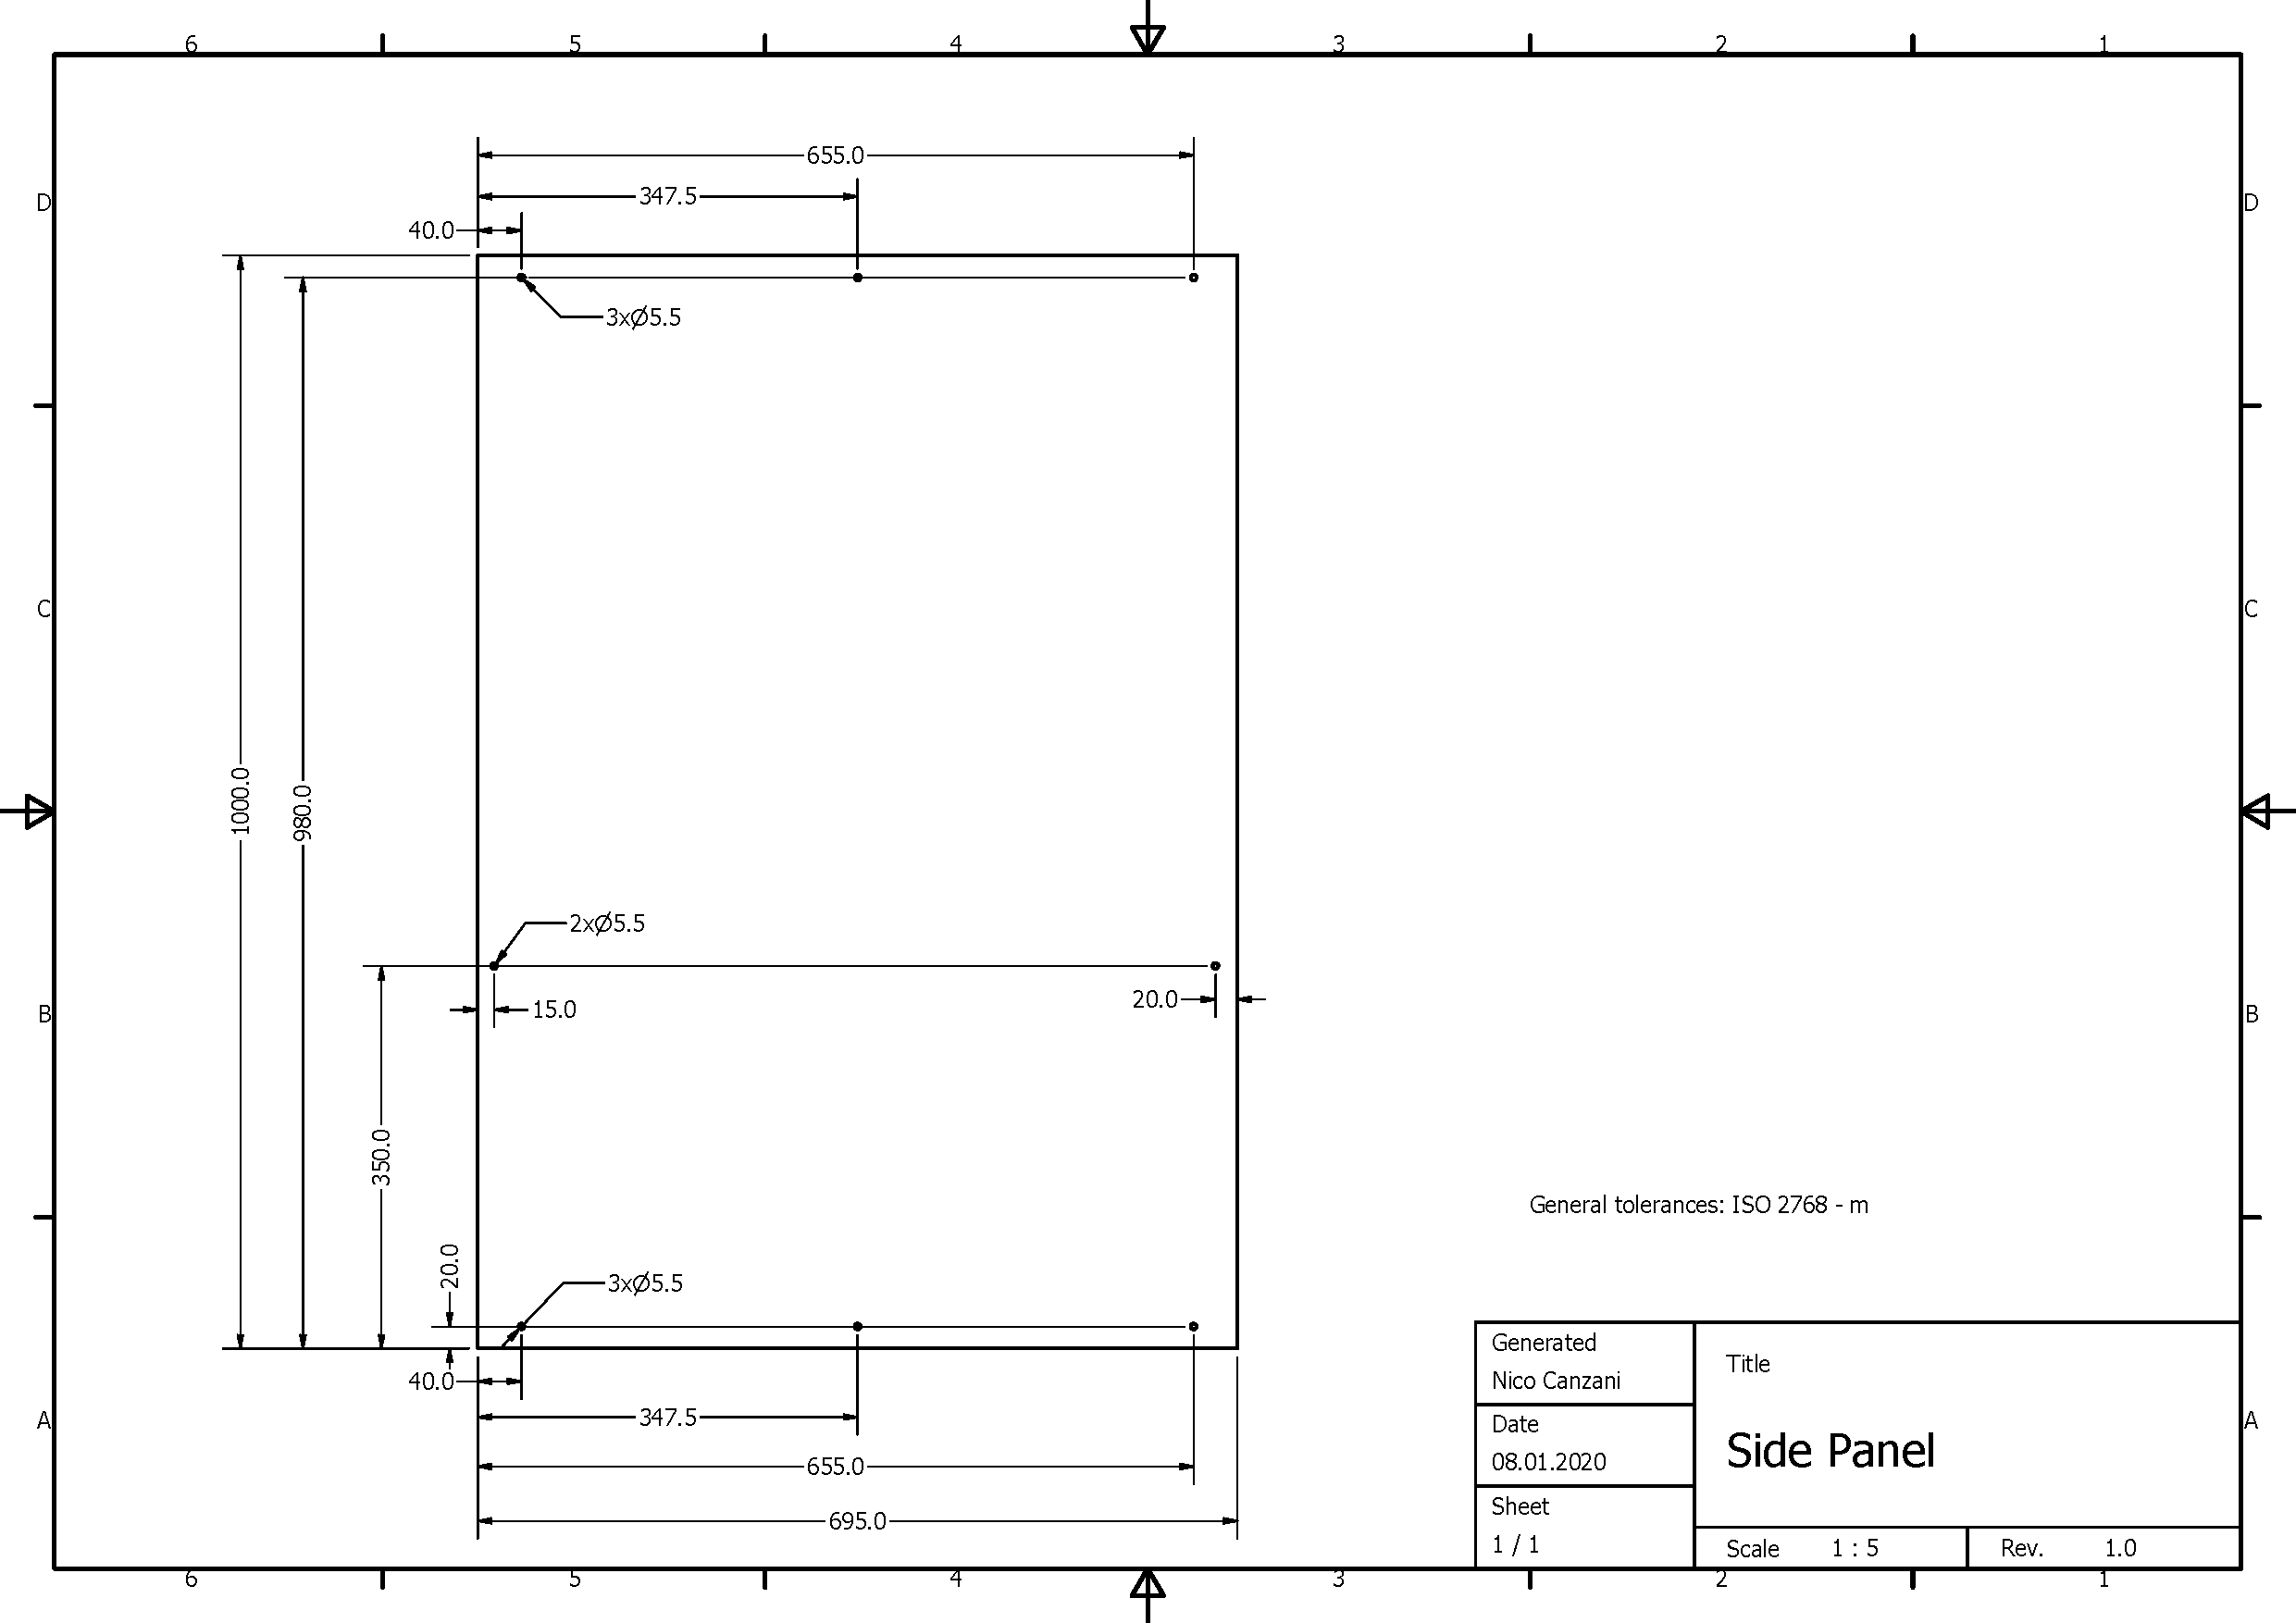
\includepdf[pages=-,landscape=true]{appendix/drawings_side_panel.pdf}

  \section{Throw Detection}
  \label{app:throw_detection}
  \lstinputlisting[style=C++]{appendix/throw_detection.cc}
\end{appendix}


% Debug
%\newpage
%\listoftodos[\section{To-Do}]
%\clearpage

\end{document}
